\documentclass[floatfix,prb,aps,superscriptaddress,11pt,preprint,letterpaper]{revtex4}
\usepackage{amsfonts}
\usepackage{amsmath}
\usepackage{graphicx}
\allowdisplaybreaks[1]%biutiful equation breaker!!!
\usepackage{ulem}
\usepackage{subfigure}
%%%%%% defs
%%%% acronimos
\def\copyr{$^\copyright$}
\def\reg{\textsuperscript{\textregistered}}
\def\tm{\textsuperscript{\texttrademark}}
\def\lufac{LUFAC${^\textsuperscript{\textregistered}}$}
%\def\depe{DP${^\textsuperscript{\texttrademark}}$}
\def\depe{DP${\texttrademark}$}
\def\ps{\mathrm{ps}}
\def\lda{\mathrm{LDA}}
\def\rpa{\mathrm{RPA}}
\def\nl{\mathrm{nl}}
\def\acu{Accu-Check\textsuperscript{\textregistered}~Performa}
\def\goni{Glucometro \'Optico No Invasivo}
\def\Reg{\textsuperscript{\textregistered}}
\def\tiniba{TINIBA\textsuperscript{\textregistered}}
\def\gw{{\it GW}}
\def\gsa{Generaci\'on del Segundo Arm\'onico}
\def\shg{Second Harmonic Generation}
\def\sfg{Sum Frequency Generation}
\def\sdf{Generaci\'on de Suma de Frecuencias}
%%%%% accent of i
\def\'#1{\if#1i{\accent19\i}\else{\accent19#1}\fi}
%%%%% compa\~nias
\def\micro{{\it Supermicro}}
%%%%% lugares
\def\lou{Laboratorio de \'Optica Ultrar\'apida}
\def\roma{Universidad de Roma II}
\def\tor{``Tor Vergata''}
\def\dti{Direcci\'on de Tecnolog\'{\i}a e Innovaci\'on}
\def\dfa{Direcci\'on de Formaci\'on Acd\'emica}
\def\dg{Direcci\'on General}
\def\da{Direcci\'on Administrativa}
\def\ifug{Insituto de F\'isica de la U. de Guanajuato}
\def\icf{Instituto de Ciencias F\'isicas}
\def\unam{Universidad Nacional Aut\'onoma de M\'exico}
\def\uguille{Universidad del Nordeste, Argentina}
\def\fotonica{Departamento de Fotonica}
\def\grupo{Propiedades \'Opticas de Nano-Sistemas, Interfases y Superficies}
\def\grupoa{PRONASIS}
%\def\grupo{Propiedades \'Opticas de Superficies e Interfases y Sistemas Nanosc\'opicos}
%\def\grupoa{POSISNA}
\def\di{Direcci\'on de Investigaci\'on}
\def\dfa{Direcci\'on de Formaci\'on Acad\'emica}
\def\cio{Centro de Investigaciones en \'Optica}
\def\ciod{Centro de Investigaciones en \'Optica, León, Guanajuato.}
\def\Conacyt{Consejo Nacional de Ciencia y Tecnolog\'ia}
\def\Concyteg{Consejo  de Ciencia y Tecnolog\'ia del Estado de Guanajuato}
\def\conacyt{CONACyT}
\def\concyteg{CONCyTEG}
\def\lagos{Centro Universitario de los Lagos}
\def\udeg{Universidad de Guadalajara}
\def\dinv{Direcci\'on de Investigaci\'on}
\def\dop{Department of Physics}
\def\uoft{University of Toronto}
\def\ua{University of Texas at Austin}
\def\icf{Instituto de Ciencias Físicas, UNAM, Cuernavaca}
%%%%% gente
%% grupo
\def\gabriel{Gabriel Ramos Ortíz}
\def\ramon{Ram\'on~ Carriles~ Jaimes}
\def\ramonm{Ram\acute{o}n~ Carriles~ Jaimes}
\def\enrique{Enrique~ Castro~ Camus}
\def\raul{Ra\'ul Alfonso V\'azquez Nava}
\def\raulm{Ra\acute{u}l~ Alfonso~ V\acute{a}zquez~ Nava}
\def\beto{Norberto~ Arzate~ Plata}
\def\bmsa{Bernardo S. Mendoza}
\def\bms{Bernardo~ Mendoza~ Santoyo}
%% alumnos
\def\cesar{C\'esar Castillo Quevedo}
\def\cabellos{Jos\'e Luis Cabellos Quiroz}
\def\tona{Tonatiuh Rangel Gordillo}
\def\temok{Juan Cuauhtemoc Salazar Gonz\'alez}
\def\adan{Luis Adan Mart\'inez Jim\'enez}
\def\sean{Sean Martin Anderson}
\def\reinaldo{Reinaldo Zapata Pe\~na}
%%% alumnos del grupo
%% enrique
%Maestria:
\def\jorgee{Jorge Alberto Caballero Mendoza}
\def\sofia{Sofía Carolina Corzo García}
\def\ruth{Ruth Julieta Medina López} 
%Doctorado: 
\def\juane{Juan Jes\'us S\'anchez S\'anchez}
%Licenciatura
\def\alma{Alma Gabriela González Patlán}
%(con Ramon): 
\def\sergioer{Sergio Augusto Romero Serv\'{\i}n}
%% Raul
%Maestria:
\def\enriquer{Enrique Arag\'on Navarro}%udg
\def\salomonr{Salom\'on Rodr\'{\i}guez Carrera}
\def\hectorr{H\'ector Santiago Hern\'andez}
\def\victor{Victor Manuel Villanueva Reyes}
%% Ramon
%Maestria:
\def\alfredora{Alfredo Campos Mej\'{\i}a}
%% Beto
%Doctorado
\def\noe{No\'e Gonz\'alez Baquedano}
%% otros
\def\liliana{Liliana Wilson Herr\'an}
\def\gerardo{Gerardo E. S\'anchez Garc\'{\i}a Rojas}
\def\amalia{Amalia Mart\'inez Garc\'{\i}a}
\def\nacho{Ing. José Ignacio Diego Manrique}
\def\tere{Teresita del Niño Jesús Pérez Hernández}
\def\elder{Elder de la Rosa Cruz}
\def\gonzalo{Gonzalo P\'aez Padilla}
\def\wlm{W. Luis Moch\'an Backal}
\def\oracio{Oracio C. Barbosa Garc\'ia}
\def\hector{H\'ector Hugo S\'anchez Hern\'andez}
\def\marco{Marco Antonio Escobar-Acevedo}
\def\gil{Alejandro Gil-Villegas Montiel}
\def\ernesto{Ernesto Carlos Cort\'es Morales}
\def\fms{Fernando Mendoza Santoyo}
\def\cuevas{Francisco Javier Cuevas de la Rosa}
\def\brenda{Brenda Esmeralda Matr\'inez Z\'erega}
\def\guille{Guillermo Ortiz}
\def\cesar{Cesar Castillo Quevedo}
\def\sipe{Prof. John Sipe}
\def\mike{Prof. Michael Downer}
\def\jems{Jorge Enrique Mej\'ia S\'anchez}
\def\lamon{Ram\'on Rodr\'iguez Vera}
\def\ldp{Luis de la Pe\~na}
\def\sole{Rodolfo Del Sole}
\def\lucia{Lucia Reining}
\def\sch{Schr\"odinger}
\def\Cuevas{Francisco J. Cuevas de la Rosa}
%%%%% categorias
\def\ita{Investigador Titular A}
\def\itb{Investigador Titular B}
\def\itc{Investigador Titular C}
\def\itd{Investigador Titular D}
\def\ite{Investigador Titular E}
\def\sr{Senior Researcher}
\def\iac{Investigador Asociado C}    
\def\alm{Alumno de Maestr\'ia}
\def\ald{Alumno de Doctorado}
\def\all{Alumno de Licenciatura}
\def\adei{Asistente de Investigaci\'on}
\def\sniIII{S.N.I. nivel III}
\def\sni{S.N.I.}
\def\cv{Currículum Vitae}
%%%%%% fonts
\def\tit{\sf}
\def\col{\sc}
\def\alu{\it} % for students
\def\cual{2$^{do}$}
\def\anno{2005}
\def\spe{\vspace{.12cm}}
%%%%%% cosas
\def\capa{capa-a-capa}
\def\espin{espintr\'onica}
\def\oespin{optoespintr\'onica}
\def\proyecto{Photon Assisted Spintronics}
\def\npro{48915}
\def\cvk{cv\mathbf{k}}
\def\cvkp{c'v'\mathbf{k}'}
%%%%%% revistas
\def\prb{Physical Review B}
\def\prl{Physical Review Letters}
\def\ol{Optics Letters}
\def\opn{Optics and Photonics News}
\def\pssc{physica status solidi (c)}
%%%%%%%%%%%%%%%%%%%%%%%%%%%%%%%%%%%%%%%
%%%%%% griegas
\def\ga{\alpha}
\def\gb{\beta}
\def\gga{\gamma}
\def\gGa{\Gamma}
\def\go{\omega}
\def\got{\tilde\omega}
\def\gO{\Omega}
\def\gr{{\rho}}
\def\ge{\epsilon}
\def\ve{\varepsilon}
\def\gve{\varepsilon}
\def\gd{\delta}
\def\gD{\Delta}
\def\gl{\lambda}
\def\gs{\sigma}
\def\gS{\Sigma}
\def\gbs{\overline{\sigma}}
\def\gka{\kappa}
%%%%%% griegas with tilde
\def\gta{\tilde{\alpha}}
\def\gtb{\tilde{\beta}}
\def\gtga{\tilde{\gamma}}
\def\gto{\tilde{\omega}}
\def\gtO{\tilde{\Omega}}
\def\gtr{\tilde{\rho}}
\def\gte{\tilde{\epsilon}}
\def\vte{\tilde{\varepsilon}}
\def\gtd{\tilde{\delta}}
\def\gtD{\tilde{\Delta}}
\def\gtl{\tilde{\lambda}}
\def\gts{\tilde{\sigma}}
\def\gtS{\tilde{\Sigma}}
%%%%%% romans with tilde
\def\bftr{\tilde{\mathbf{r}}}
\def\bftp{\tilde{\mathbf{p}}}
\def\bftv{\tilde{\mathbf{v}}}
\def\ta{\tilde{a}}
\def\tb{\tilde{b}}
\def\tr{\tilde{r}}
\def\tp{\tilde{p}}
\def\tV{\tilde{V}}
\def\tv{\tilde{v}}
%%
\newcommand{\ham}{\hat{\mathcal H}}
%%%%%% bra kets
\newcommand{\la}{\langle}
\newcommand{\ra}{\rangle}
\newcommand{\ket}[1]{| #1 \rangle}
\newcommand{\bra}[1]{\langle #1 |}
\newcommand{\braket}[2]{\langle {#1} | {#2} \rangle}
\newcommand{\ketbra}[2]{| {#1} \rangle {#1} \langle {#2} |}
\newcommand{\ave}[1]{\langle {#1} \rangle}
\newcommand{\dotp}[2]{\mathbf{#1} \cdot \mathbf{#2}}
%%%%%% averages
\newcommand{\prom}[1]{\langle {#1} \rangle}
%%%%%% creation and annihilation operators
\newcommand{\oa}{\hat a^{\tiny\strut}}
\newcommand{\oad}{\hat a^\dagger}
\newcommand{\oadk}{\hat a^\dagger_{\mathbf k}}
\newcommand{\oak}{\hat a^{\tiny\strut}_{\mathbf k}}
\newcommand{\obd}[1]{\hat b^\dagger_{#1}}
\newcommand{\ob}[1]{\hat b^{\tiny\strut}_{#1}}
%%%%%% Caligraphic
\newcommand{\cala}{{\mathbf{\cal A}}}
\newcommand{\calb}{{\mathbf{\cal B}}}
\newcommand{\calc}{{\mathbf{\cal C}}}
\newcommand{\cald}{{\mathbf{\cal D}}}
\newcommand{\cale}{{\mathbf{\cal E}}}
\newcommand{\calf}{{\mathbf{\cal F}}}
\newcommand{\calh}{{\mathbf{\cal H}}}
\newcommand{\cali}{{\mathbf{\cal I}}}
\newcommand{\calp}{{\mathbf{\cal P}}}
\newcommand{\calg}{{\mathbf{\cal G}}}
\newcommand{\calv}{{\mathbf{\cal V}}}
\newcommand{\call}{{\cal L}}
\newcommand{\calo}{{\cal O}}
\newcommand{\caln}{{\cal N}}
\newcommand{\calr}{{\cal R}}
\newcommand{\cals}{{\cal S}}
\newcommand{\calt}{{\cal T}}
\newcommand{\calu}{{\cal U}}
\newcommand{\calw}{{\cal W}}
\newcommand{\calbd}{\boldsymbol{\mathcal{\cal D}}}
\newcommand{\calbp}{\boldsymbol{\mathcal{\cal P}}}
\newcommand{\calbv}{\boldsymbol{\mathcal{\cal V}}}
\newcommand{\calbs}{\boldsymbol{\mathcal{\cal S}}}
\newcommand{\calbg}{\boldsymbol{\mathcal{\cal G}}}
%%%%%% mathematicla bold roman & greek
\newcommand{\mbf}[1]{\mathbf{#1}}
\newcommand{\mbg}[1]{\boldsymbol{\mathcal {#1}}}
\newcommand{\bfA}{\mathbf{A}}
\newcommand{\bfB}{\mathbf{B}}
\newcommand{\bfC}{\mathbf{C}}
\newcommand{\bfD}{\mathbf{D}}
\newcommand{\bfE}{\mathbf{E}}
\newcommand{\bfF}{\mathbf{F}}
\newcommand{\bfG}{\mathbf{G}}
\newcommand{\bfH}{\mathbf{H}}
\newcommand{\bfI}{\mathbf{I}}
\newcommand{\bfJ}{\mathbf{J}}
\newcommand{\bfK}{\mathbf{K}}
\newcommand{\bfL}{\mathbf{L}}
\newcommand{\bfM}{\mathbf{M}}
\newcommand{\bfN}{\mathbf{N}}
\newcommand{\bfP}{\mathbf{P}}
\newcommand{\bfR}{\mathbf{R}}
\newcommand{\bfS}{\mathbf{S}}
\newcommand{\bfT}{\mathbf{T}}
\newcommand{\bfU}{\mathbf{U}}
\newcommand{\bfV}{\mathbf{V}}
\newcommand{\bfW}{\mathbf{W}}
\newcommand{\bfX}{\mathbf{X}}
\newcommand{\bfY}{\mathbf{Y}}
\newcommand{\bfZ}{\mathbf{Z}}
\newcommand{\bfa}{\mathbf{a}}
\newcommand{\bfb}{\mathbf{b}}
\newcommand{\bfc}{\mathbf{c}}
\newcommand{\bfd}{\mathbf{d}}
\newcommand{\bfe}{\mathbf{e}}
\newcommand{\bff}{\mathbf{f}}
\newcommand{\bfg}{\mathbf{g}}
\newcommand{\bfh}{\mathbf{h}}
\newcommand{\bfi}{\mathbf{i}}
\newcommand{\bfj}{\mathbf{j}}
\newcommand{\bfk}{\mathbf{k}}
\newcommand{\bfn}{\mathbf{n}}
\newcommand{\bfp}{\mathbf{p}}
\newcommand{\bfq}{\mathbf{q}}
\newcommand{\bfr}{\mathbf{r}}
\newcommand{\bfs}{\mathbf{s}}
\newcommand{\bft}{\mathbf{t}}
\newcommand{\bfu}{\mathbf{u}}
\newcommand{\bfv}{\mathbf{v}}
\newcommand{\bfx}{\mathbf{x}}
\newcommand{\bfy}{\mathbf{y}}
\newcommand{\bfz}{\mathbf{z}}
\newcommand{\bfzero}{\mathbf{0}}
\newcommand{\bfone}{\mathbf{1}}
%
\newcommand{\bfgeta}{\boldsymbol{\eta}}
\newcommand{\bfSig}{\boldsymbol{\Sigma}}
\newcommand{\bfsig}{\boldsymbol{\sigma}}
\newcommand{\bfgS}{\boldsymbol{\Sigma}}
\newcommand{\bfgs}{\boldsymbol{\sigma}}
\newcommand{\bfga}{\boldsymbol{\alpha}}
\newcommand{\bfgb}{\boldsymbol{\beta}}
\newcommand{\bfge}{\boldsymbol{\epsilon}}
\newcommand{\bfgvare}{\boldsymbol{\varepsilon}}
\newcommand{\bfgg}{\boldsymbol{\gamma}}
\newcommand{\bfgG}{\boldsymbol{\Gamma}}
\newcommand{\bfgphi}{\boldsymbol{\phi}}
\newcommand{\bfgpsi}{\boldsymbol{\psi}}
\newcommand{\bfgD}{\boldsymbol{\Delta}}
\newcommand{\bfgPhi}{\boldsymbol{\Phi}}
\newcommand{\bfgPsi}{\boldsymbol{\Psi}}
\newcommand{\bfgtau}{\boldsymbol{\tau}}
\newcommand{\bfgxi}{\boldsymbol{\xi}}
\newcommand{\bfgchi}{\boldsymbol{\chi}}
\newcommand{\bfgnabla}{\boldsymbol{\nabla}}
\newcommand{\bfgnu}{\boldsymbol{\nu}}
\newcommand{\bfgmu}{\boldsymbol{\mu}}
\newcommand{\bfgrho}{\boldsymbol{\rho}}
\newcommand{\bfgRho}{\boldsymbol{\Rho}}
%%%%%% nabla
\newcommand{\nablak}{\frac{\partial}{\partial\mathbf{k}} }
%%%%%% ; derivative
\def\gk{{;\mathbf k}}
%%%%%% k derivative
\newcommand{\deriv}[2] {\frac{\partial {#1}} {\partial {#2} }}
%%%%%% prime for \sum
\def\prima{\strut^{_{'}}}
%%%%%% subindices
%\def\eti{n\bfk}
\newcommand{\eti}[1]{_{#1 \bfk}}
\newcommand{\etiup}[1]{_{#1 \bfk s}}
\newcommand{\etidn}[1]{_{#1 \bfk \bar{s}}}
%%%%% superindice to push down the subindex in greeks!
\def\pd{^{\strut}}
%%%%% gauges
\def\rde{$\bfr\cdot\bfE$~}
\def\rder{length-gauge}
\def\pda{$\bfp\cdot\bfA$~}
\def\vda{$\bfv\cdot\bfA$~}
\def\vdar{velocity-gauge}
%%%%% integral over k
\def\intk{\int\frac{d^3k}{8\pi^3}}
%%%%% roman indices
\def\rmi{\mathrm{i}}
\def\rmj{\mathrm{j}}
\def\rmk{\mathrm{k}}
\def\rml{\mathrm{l}}
\def\rmr{\mathrm{r}}
\def\rma{\mathrm{a}}
\def\rmb{\mathrm{b}}
\def\rmc{\mathrm{c}}
\def\rmd{\mathrm{d}}
\def\rme{\mathrm{e}}
\def\rmv{\mathrm{v}}
\def\rmz{\mathrm{z}}
\def\rmx{\mathrm{x}}
\def\rmy{\mathrm{y}}
\def\rmH{\mathrm{H}}
\def\rmI{\mathrm{I}}
\def\rmG{\mathrm{G}}
\def\rmW{\mathrm{W}}
%%%%% functions
\def\erf{\mathrm{erf}}
\def\erfc{\mathrm{erfc}}
\def\erfi{\mathrm{erfi}}

%iave: C01243171 y 0124317111
%%%%% Green's one point model
\def\tyv{\tilde y_v}
\def\ty{\tilde y}
\def\tv{\tilde v}

%\def\chon[1]{\color{red} #1}
\def\chon{red}
\def\chonn{red}
\def\nicolas{red}
%%%%% defs
%%%% acronimos
\def\copyr{$^\copyright$}
\def\reg{\textsuperscript{\textregistered}}
\def\tm{\textsuperscript{\texttrademark}}
\def\lufac{LUFAC${^\textsuperscript{\textregistered}}$}
%\def\depe{DP${^\textsuperscript{\texttrademark}}$}
\def\depe{DP${\texttrademark}$}
\def\ps{\mathrm{ps}}
\def\lda{\mathrm{LDA}}
\def\rpa{\mathrm{RPA}}
\def\nl{\mathrm{nl}}
\def\acu{Accu-Check\textsuperscript{\textregistered}~Performa}
\def\goni{Glucometro \'Optico No Invasivo}
\def\Reg{\textsuperscript{\textregistered}}
\def\tiniba{TINIBA\textsuperscript{\textregistered}}
\def\gw{{\it GW}}
\def\gsa{Generaci\'on del Segundo Arm\'onico}
\def\shg{Second Harmonic Generation}
\def\sfg{Sum Frequency Generation}
\def\sdf{Generaci\'on de Suma de Frecuencias}
%%%%% accent of i
\def\'#1{\if#1i{\accent19\i}\else{\accent19#1}\fi}
%%%%% compa\~nias
\def\micro{{\it Supermicro}}
%%%%% lugares
\def\lou{Laboratorio de \'Optica Ultrar\'apida}
\def\roma{Universidad de Roma II}
\def\tor{``Tor Vergata''}
\def\dti{Direcci\'on de Tecnolog\'{\i}a e Innovaci\'on}
\def\dfa{Direcci\'on de Formaci\'on Acd\'emica}
\def\dg{Direcci\'on General}
\def\da{Direcci\'on Administrativa}
\def\ifug{Insituto de F\'isica de la U. de Guanajuato}
\def\icf{Instituto de Ciencias F\'isicas}
\def\unam{Universidad Nacional Aut\'onoma de M\'exico}
\def\uguille{Universidad del Nordeste, Argentina}
\def\fotonica{Departamento de Fotonica}
\def\grupo{Propiedades \'Opticas de Nano-Sistemas, Interfases y Superficies}
\def\grupoa{PRONASIS}
%\def\grupo{Propiedades \'Opticas de Superficies e Interfases y Sistemas Nanosc\'opicos}
%\def\grupoa{POSISNA}
\def\di{Direcci\'on de Investigaci\'on}
\def\dfa{Direcci\'on de Formaci\'on Acad\'emica}
\def\cio{Centro de Investigaciones en \'Optica}
\def\ciod{Centro de Investigaciones en \'Optica, León, Guanajuato.}
\def\Conacyt{Consejo Nacional de Ciencia y Tecnolog\'ia}
\def\Concyteg{Consejo  de Ciencia y Tecnolog\'ia del Estado de Guanajuato}
\def\conacyt{CONACyT}
\def\concyteg{CONCyTEG}
\def\lagos{Centro Universitario de los Lagos}
\def\udeg{Universidad de Guadalajara}
\def\dinv{Direcci\'on de Investigaci\'on}
\def\dop{Department of Physics}
\def\uoft{University of Toronto}
\def\ua{University of Texas at Austin}
\def\icf{Instituto de Ciencias Físicas, UNAM, Cuernavaca}
%%%%% gente
%% grupo
\def\gabriel{Gabriel Ramos Ortíz}
\def\ramon{Ram\'on~ Carriles~ Jaimes}
\def\ramonm{Ram\acute{o}n~ Carriles~ Jaimes}
\def\enrique{Enrique~ Castro~ Camus}
\def\raul{Ra\'ul Alfonso V\'azquez Nava}
\def\raulm{Ra\acute{u}l~ Alfonso~ V\acute{a}zquez~ Nava}
\def\beto{Norberto~ Arzate~ Plata}
\def\bmsa{Bernardo S. Mendoza}
\def\bms{Bernardo~ Mendoza~ Santoyo}
%% alumnos
\def\cesar{C\'esar Castillo Quevedo}
\def\cabellos{Jos\'e Luis Cabellos Quiroz}
\def\tona{Tonatiuh Rangel Gordillo}
\def\temok{Juan Cuauhtemoc Salazar Gonz\'alez}
\def\adan{Luis Adan Mart\'inez Jim\'enez}
\def\sean{Sean Martin Anderson}
\def\reinaldo{Reinaldo Zapata Pe\~na}
%%% alumnos del grupo
%% enrique
%Maestria:
\def\jorgee{Jorge Alberto Caballero Mendoza}
\def\sofia{Sofía Carolina Corzo García}
\def\ruth{Ruth Julieta Medina López} 
%Doctorado: 
\def\juane{Juan Jes\'us S\'anchez S\'anchez}
%Licenciatura
\def\alma{Alma Gabriela González Patlán}
%(con Ramon): 
\def\sergioer{Sergio Augusto Romero Serv\'{\i}n}
%% Raul
%Maestria:
\def\enriquer{Enrique Arag\'on Navarro}%udg
\def\salomonr{Salom\'on Rodr\'{\i}guez Carrera}
\def\hectorr{H\'ector Santiago Hern\'andez}
\def\victor{Victor Manuel Villanueva Reyes}
%% Ramon
%Maestria:
\def\alfredora{Alfredo Campos Mej\'{\i}a}
%% Beto
%Doctorado
\def\noe{No\'e Gonz\'alez Baquedano}
%% otros
\def\liliana{Liliana Wilson Herr\'an}
\def\gerardo{Gerardo E. S\'anchez Garc\'{\i}a Rojas}
\def\amalia{Amalia Mart\'inez Garc\'{\i}a}
\def\nacho{Ing. José Ignacio Diego Manrique}
\def\tere{Teresita del Niño Jesús Pérez Hernández}
\def\elder{Elder de la Rosa Cruz}
\def\gonzalo{Gonzalo P\'aez Padilla}
\def\wlm{W. Luis Moch\'an Backal}
\def\oracio{Oracio C. Barbosa Garc\'ia}
\def\hector{H\'ector Hugo S\'anchez Hern\'andez}
\def\marco{Marco Antonio Escobar-Acevedo}
\def\gil{Alejandro Gil-Villegas Montiel}
\def\ernesto{Ernesto Carlos Cort\'es Morales}
\def\fms{Fernando Mendoza Santoyo}
\def\cuevas{Francisco Javier Cuevas de la Rosa}
\def\brenda{Brenda Esmeralda Matr\'inez Z\'erega}
\def\guille{Guillermo Ortiz}
\def\cesar{Cesar Castillo Quevedo}
\def\sipe{Prof. John Sipe}
\def\mike{Prof. Michael Downer}
\def\jems{Jorge Enrique Mej\'ia S\'anchez}
\def\lamon{Ram\'on Rodr\'iguez Vera}
\def\ldp{Luis de la Pe\~na}
\def\sole{Rodolfo Del Sole}
\def\lucia{Lucia Reining}
\def\sch{Schr\"odinger}
\def\Cuevas{Francisco J. Cuevas de la Rosa}
%%%%% categorias
\def\ita{Investigador Titular A}
\def\itb{Investigador Titular B}
\def\itc{Investigador Titular C}
\def\itd{Investigador Titular D}
\def\ite{Investigador Titular E}
\def\sr{Senior Researcher}
\def\iac{Investigador Asociado C}    
\def\alm{Alumno de Maestr\'ia}
\def\ald{Alumno de Doctorado}
\def\all{Alumno de Licenciatura}
\def\adei{Asistente de Investigaci\'on}
\def\sniIII{S.N.I. nivel III}
\def\sni{S.N.I.}
\def\cv{Currículum Vitae}
%%%%%% fonts
\def\tit{\sf}
\def\col{\sc}
\def\alu{\it} % for students
\def\cual{2$^{do}$}
\def\anno{2005}
\def\spe{\vspace{.12cm}}
%%%%%% cosas
\def\capa{capa-a-capa}
\def\espin{espintr\'onica}
\def\oespin{optoespintr\'onica}
\def\proyecto{Photon Assisted Spintronics}
\def\npro{48915}
\def\cvk{cv\mathbf{k}}
\def\cvkp{c'v'\mathbf{k}'}
%%%%%% revistas
\def\prb{Physical Review B}
\def\prl{Physical Review Letters}
\def\ol{Optics Letters}
\def\opn{Optics and Photonics News}
\def\pssc{physica status solidi (c)}
%%%%%%%%%%%%%%%%%%%%%%%%%%%%%%%%%%%%%%%
%%%%%% griegas
\def\ga{\alpha}
\def\gb{\beta}
\def\gga{\gamma}
\def\gGa{\Gamma}
\def\go{\omega}
\def\got{\tilde\omega}
\def\gO{\Omega}
\def\gr{{\rho}}
\def\ge{\epsilon}
\def\ve{\varepsilon}
\def\gve{\varepsilon}
\def\gd{\delta}
\def\gD{\Delta}
\def\gl{\lambda}
\def\gs{\sigma}
\def\gS{\Sigma}
\def\gbs{\overline{\sigma}}
\def\gka{\kappa}
%%%%%% griegas with tilde
\def\gta{\tilde{\alpha}}
\def\gtb{\tilde{\beta}}
\def\gtga{\tilde{\gamma}}
\def\gto{\tilde{\omega}}
\def\gtO{\tilde{\Omega}}
\def\gtr{\tilde{\rho}}
\def\gte{\tilde{\epsilon}}
\def\vte{\tilde{\varepsilon}}
\def\gtd{\tilde{\delta}}
\def\gtD{\tilde{\Delta}}
\def\gtl{\tilde{\lambda}}
\def\gts{\tilde{\sigma}}
\def\gtS{\tilde{\Sigma}}
%%%%%% romans with tilde
\def\bftr{\tilde{\mathbf{r}}}
\def\bftp{\tilde{\mathbf{p}}}
\def\bftv{\tilde{\mathbf{v}}}
\def\ta{\tilde{a}}
\def\tb{\tilde{b}}
\def\tr{\tilde{r}}
\def\tp{\tilde{p}}
\def\tV{\tilde{V}}
\def\tv{\tilde{v}}
%%
\newcommand{\ham}{\hat{\mathcal H}}
%%%%%% bra kets
\newcommand{\la}{\langle}
\newcommand{\ra}{\rangle}
\newcommand{\ket}[1]{| #1 \rangle}
\newcommand{\bra}[1]{\langle #1 |}
\newcommand{\braket}[2]{\langle {#1} | {#2} \rangle}
\newcommand{\ketbra}[2]{| {#1} \rangle {#1} \langle {#2} |}
\newcommand{\ave}[1]{\langle {#1} \rangle}
\newcommand{\dotp}[2]{\mathbf{#1} \cdot \mathbf{#2}}
%%%%%% averages
\newcommand{\prom}[1]{\langle {#1} \rangle}
%%%%%% creation and annihilation operators
\newcommand{\oa}{\hat a^{\tiny\strut}}
\newcommand{\oad}{\hat a^\dagger}
\newcommand{\oadk}{\hat a^\dagger_{\mathbf k}}
\newcommand{\oak}{\hat a^{\tiny\strut}_{\mathbf k}}
\newcommand{\obd}[1]{\hat b^\dagger_{#1}}
\newcommand{\ob}[1]{\hat b^{\tiny\strut}_{#1}}
%%%%%% Caligraphic
\newcommand{\cala}{{\mathbf{\cal A}}}
\newcommand{\calb}{{\mathbf{\cal B}}}
\newcommand{\calc}{{\mathbf{\cal C}}}
\newcommand{\cald}{{\mathbf{\cal D}}}
\newcommand{\cale}{{\mathbf{\cal E}}}
\newcommand{\calf}{{\mathbf{\cal F}}}
\newcommand{\calh}{{\mathbf{\cal H}}}
\newcommand{\cali}{{\mathbf{\cal I}}}
\newcommand{\calp}{{\mathbf{\cal P}}}
\newcommand{\calg}{{\mathbf{\cal G}}}
\newcommand{\calv}{{\mathbf{\cal V}}}
\newcommand{\call}{{\cal L}}
\newcommand{\calo}{{\cal O}}
\newcommand{\caln}{{\cal N}}
\newcommand{\calr}{{\cal R}}
\newcommand{\cals}{{\cal S}}
\newcommand{\calt}{{\cal T}}
\newcommand{\calu}{{\cal U}}
\newcommand{\calw}{{\cal W}}
\newcommand{\calbd}{\boldsymbol{\mathcal{\cal D}}}
\newcommand{\calbp}{\boldsymbol{\mathcal{\cal P}}}
\newcommand{\calbv}{\boldsymbol{\mathcal{\cal V}}}
\newcommand{\calbs}{\boldsymbol{\mathcal{\cal S}}}
\newcommand{\calbg}{\boldsymbol{\mathcal{\cal G}}}
%%%%%% mathematicla bold roman & greek
\newcommand{\mbf}[1]{\mathbf{#1}}
\newcommand{\mbg}[1]{\boldsymbol{\mathcal {#1}}}
\newcommand{\bfA}{\mathbf{A}}
\newcommand{\bfB}{\mathbf{B}}
\newcommand{\bfC}{\mathbf{C}}
\newcommand{\bfD}{\mathbf{D}}
\newcommand{\bfE}{\mathbf{E}}
\newcommand{\bfF}{\mathbf{F}}
\newcommand{\bfG}{\mathbf{G}}
\newcommand{\bfH}{\mathbf{H}}
\newcommand{\bfI}{\mathbf{I}}
\newcommand{\bfJ}{\mathbf{J}}
\newcommand{\bfK}{\mathbf{K}}
\newcommand{\bfL}{\mathbf{L}}
\newcommand{\bfM}{\mathbf{M}}
\newcommand{\bfN}{\mathbf{N}}
\newcommand{\bfP}{\mathbf{P}}
\newcommand{\bfR}{\mathbf{R}}
\newcommand{\bfS}{\mathbf{S}}
\newcommand{\bfT}{\mathbf{T}}
\newcommand{\bfU}{\mathbf{U}}
\newcommand{\bfV}{\mathbf{V}}
\newcommand{\bfW}{\mathbf{W}}
\newcommand{\bfX}{\mathbf{X}}
\newcommand{\bfY}{\mathbf{Y}}
\newcommand{\bfZ}{\mathbf{Z}}
\newcommand{\bfa}{\mathbf{a}}
\newcommand{\bfb}{\mathbf{b}}
\newcommand{\bfc}{\mathbf{c}}
\newcommand{\bfd}{\mathbf{d}}
\newcommand{\bfe}{\mathbf{e}}
\newcommand{\bff}{\mathbf{f}}
\newcommand{\bfg}{\mathbf{g}}
\newcommand{\bfh}{\mathbf{h}}
\newcommand{\bfi}{\mathbf{i}}
\newcommand{\bfj}{\mathbf{j}}
\newcommand{\bfk}{\mathbf{k}}
\newcommand{\bfn}{\mathbf{n}}
\newcommand{\bfp}{\mathbf{p}}
\newcommand{\bfq}{\mathbf{q}}
\newcommand{\bfr}{\mathbf{r}}
\newcommand{\bfs}{\mathbf{s}}
\newcommand{\bft}{\mathbf{t}}
\newcommand{\bfu}{\mathbf{u}}
\newcommand{\bfv}{\mathbf{v}}
\newcommand{\bfx}{\mathbf{x}}
\newcommand{\bfy}{\mathbf{y}}
\newcommand{\bfz}{\mathbf{z}}
\newcommand{\bfzero}{\mathbf{0}}
\newcommand{\bfone}{\mathbf{1}}
%
\newcommand{\bfgeta}{\boldsymbol{\eta}}
\newcommand{\bfSig}{\boldsymbol{\Sigma}}
\newcommand{\bfsig}{\boldsymbol{\sigma}}
\newcommand{\bfgS}{\boldsymbol{\Sigma}}
\newcommand{\bfgs}{\boldsymbol{\sigma}}
\newcommand{\bfga}{\boldsymbol{\alpha}}
\newcommand{\bfgb}{\boldsymbol{\beta}}
\newcommand{\bfge}{\boldsymbol{\epsilon}}
\newcommand{\bfgvare}{\boldsymbol{\varepsilon}}
\newcommand{\bfgg}{\boldsymbol{\gamma}}
\newcommand{\bfgG}{\boldsymbol{\Gamma}}
\newcommand{\bfgphi}{\boldsymbol{\phi}}
\newcommand{\bfgpsi}{\boldsymbol{\psi}}
\newcommand{\bfgD}{\boldsymbol{\Delta}}
\newcommand{\bfgPhi}{\boldsymbol{\Phi}}
\newcommand{\bfgPsi}{\boldsymbol{\Psi}}
\newcommand{\bfgtau}{\boldsymbol{\tau}}
\newcommand{\bfgxi}{\boldsymbol{\xi}}
\newcommand{\bfgchi}{\boldsymbol{\chi}}
\newcommand{\bfgnabla}{\boldsymbol{\nabla}}
\newcommand{\bfgnu}{\boldsymbol{\nu}}
\newcommand{\bfgmu}{\boldsymbol{\mu}}
\newcommand{\bfgrho}{\boldsymbol{\rho}}
\newcommand{\bfgRho}{\boldsymbol{\Rho}}
%%%%%% nabla
\newcommand{\nablak}{\frac{\partial}{\partial\mathbf{k}} }
%%%%%% ; derivative
\def\gk{{;\mathbf k}}
%%%%%% k derivative
\newcommand{\deriv}[2] {\frac{\partial {#1}} {\partial {#2} }}
%%%%%% prime for \sum
\def\prima{\strut^{_{'}}}
%%%%%% subindices
%\def\eti{n\bfk}
\newcommand{\eti}[1]{_{#1 \bfk}}
\newcommand{\etiup}[1]{_{#1 \bfk s}}
\newcommand{\etidn}[1]{_{#1 \bfk \bar{s}}}
%%%%% superindice to push down the subindex in greeks!
\def\pd{^{\strut}}
%%%%% gauges
\def\rde{$\bfr\cdot\bfE$~}
\def\rder{length-gauge}
\def\pda{$\bfp\cdot\bfA$~}
\def\vda{$\bfv\cdot\bfA$~}
\def\vdar{velocity-gauge}
%%%%% integral over k
\def\intk{\int\frac{d^3k}{8\pi^3}}
%%%%% roman indices
\def\rmi{\mathrm{i}}
\def\rmj{\mathrm{j}}
\def\rmk{\mathrm{k}}
\def\rml{\mathrm{l}}
\def\rmr{\mathrm{r}}
\def\rma{\mathrm{a}}
\def\rmb{\mathrm{b}}
\def\rmc{\mathrm{c}}
\def\rmd{\mathrm{d}}
\def\rme{\mathrm{e}}
\def\rmv{\mathrm{v}}
\def\rmz{\mathrm{z}}
\def\rmx{\mathrm{x}}
\def\rmy{\mathrm{y}}
\def\rmH{\mathrm{H}}
\def\rmI{\mathrm{I}}
\def\rmG{\mathrm{G}}
\def\rmW{\mathrm{W}}
%%%%% functions
\def\erf{\mathrm{erf}}
\def\erfc{\mathrm{erfc}}
\def\erfi{\mathrm{erfi}}

%iave: C01243171 y 0124317111
%%%%% Green's one point model
\def\tyv{\tilde y_v}
\def\ty{\tilde y}
\def\tv{\tilde v}

\usepackage{bm}
%%%%*****************%%%% fine hyperef 
\usepackage[backref,pdffitwindow,colorlinks,linkcolor={blue},citecolor={red}]{hyperref}
%%%%%%%%%%%%%%%%%%%%%%%%%%%%%%%%%%%%%%%
\usepackage{showlabels}
%\usepackage{showkeys}

%%%
% notes:
% nonlocal, not non-local
% check for tense consistency
% surface SHG = SSHG
% $\bfk$-points, not $\bfk$ points
% Nature Materials de valerie
% Local fields?
%%%



\begin{document}

\title{Length Gauge Theory of Surface Second Harmonic Generation}
\author{Sean M. Anderson}
\affiliation{Centro de Investigaciones en Optica, Le\'on, Guanajuato, M\'exico}
\author{Nicolas Tancogne-Dejean}
\affiliation{Laboratoire des Solides Irradi\'es, \'Ecole 
  Polytechnique, CNRS, CEA/DSM, 91128 Palaiseau, France}
 \affiliation{European Theoretical Spectroscopy Facility (ETSF), Palaiseau, France}
\author{Bernardo S. Mendoza}\email{bms@cio.mx}
\affiliation{Centro de Investigaciones en Optica, Le\'on, Guanajuato, M\'exico}
\author{Val\'erie V\'eniard}
\affiliation{Laboratoire des Solides Irradi\'es, \'Ecole 
  Polytechnique, CNRS, CEA/DSM, 91128 Palaiseau, France}
 \affiliation{European Theoretical Spectroscopy Facility (ETSF), Palaiseau, France}

\begin{abstract}
We present a theoretical review of surface second harmonic generation (SHG) 
from semiconductor surfaces based on the length gauge. This 
layer-by-layer analysis is carefully presented in order to show how a 
surface SHG calculation can be readily evaluated. The nonlinear susceptibility 
tensor for a surface, $\boldsymbol{\chi}^S(-2\go;\go,\go)$
is split into two terms relating to inter-band 
and intra-band one-electron transitions. 

\end{abstract}  

\maketitle
%\tableofcontents

\section{Introduction}\label{intro}


In recent years, surface nonlinear optical spectroscopies and in 
particular, surface second-harmonic generation SSHG have evolved as useful 
nondestructive and noninvasive tool to study properties of surfaces 
and interfaces: atomic structure, phase transitions, and adsorption of 
atoms, among others.\cite{
    daumPRL93, 
    mcgilpOE94, 
    meyerPRL95, 
    powerPRL95, 
    godefroyAPL96, 
    hoferAPA96, 
    dadapPRB97, 
    bloembergenAPB99, 
    mcgilpSRL99, 
    suzukiAPB99, 
    mitchellSS01,
    hughesPRB96, 
    guyotPRB88, 
    downerPSSA01, 
    shenAPB99, 
    shenNAT89, 
    chenPRL81, 
    mendozaPRL98,
    downerSIA01,
    cazzanelliNM14}
Nowadays, SSHG spectroscopy is a crucial tool for research and development
in microelectronics,\cite{zheltikovLP00} semiconductors,
\cite{lupkeSSR99}, nanomaterials,\cite{salazar-aparicioPRB14} 
and many more recent 
areas of great scientific and commercial interest.\cite{cazzanelliNM14}
The high surface sensitivity of SSHG spectroscopy is due to the
fact that, within the dipole approximation, the bulk SHG signal of
centrosymmetric materials is identically zero, and thus only the
surface, where the inversion symmetry is broken, can radiate. 
Much of the foundation of surface science has been built from
experiments involving emission or scattering of electrons from
surfaces. These require ultrahigh vacuum (UHV) environments and
provide no access to buried interfaces. 
However, SSHG
is compatibile with non-UHV ambients and has access to
interfaces buried beneath transparent overlayers. Even when applied to
surfaces in UHV, the light source and detectors can be aligned and
used outside the vacuum chamber. 

The usefulness of SSHG could be limited by
the lack of microscopic theoretical
understanding of the nonlinear spectra. The macroscopic
phenomenological theory of SSHG, which relates the intensity,
phase and polarization of detected fields to nonlinear and linear
susceptibilities at the material interface, is now fully developed. 
However, microscopic theory, which relates atomic-level structure to
the nonlinear source polarization, is still being developed.
In this article we put forward an approach to calculate the
microscopic second harmonic surface susceptibility that encompasses several
theoretical features not taken into account before. 
Within the independent particle approximation (IPA),  
some frameworks for bulk SHG have been developed to study the 
nonlinear optical response of bulk materials, where several degrees of
sophistication were 
introduced.\cite{butcherPOPS63,aspnesPRB72,sipePRB93,levinePRB94,aversaPRB95,hughesPRB96,rashkeevPRB98} 

As it is well known
Density Functional Theory (DFT) within the Local Density Approximation
(LDA),\cite{kohnPR65} the most 
used framework for \textit{ab initio} calculations,
underestimates the energy band gap of semiconductors. It is also well
understood that one has to include the many-body interaction to
correct for the underestimation of the gap. In this context the so
called GW approximation\cite{onidaRMP02} is known to correct the band
gap of most semiconductors\cite{luceroJPCM12}. However this could be a numerically very
expensive calculation, and thus one uses the much simpler scissors
operator scheme.\cite{levinePRL89, levinePRL91}
This allows to ``open'' the DFT-LDA gap to
its correct experimental or GW value, when experiments are not available. 
In this context,
to correct for the underestimation of the energy band gap of semiconductors, 
Nastos et al.\cite{nastosPRB05} 
using the 
``length gauge'' or 
``$\mathbf{r}\cdot\mathbf{E}$ gauge'' 
showed how to correctly include in the SH susceptibility the many-body corrections through the
scissors operator.
Later,
Cabellos \textit{et al}.\cite{cabellosPRB09} 
elaborated a derivation of the ``velocity gauge'' or
``$\bfA\cdot\bfv$'' gauge properly including the scissors
operator, and proved  gauge 
invariance with respect to the length gauge.
From these works, it is clear the length gauge is a much better staring
point to obtain the surface SH (SSH) susceptibility, as it will be
elaborated in this article. Above only being valid for bulk semiconductors.

Concerning the optical response of surfaces and interfaces,
Reining \textit{et al.}\cite{reiningPRB94}  
introduced the concept of a 
cut function in order to obtain the surface SH 
susceptibility tensor.
This cut function is required since one usually uses a slab approach
when treating semi-infinite surface systems; if the slab is
centrosymmetric the susceptibility tensor will be identically zero.
The cut function is such that it separates the nonlinear response
the two surfaces of the slab, thus avoiding the destructive
interference between them, giving a finite value of the tensor, that
one identifies with the SSH susceptibility tensor; if the slab is not
centrosymmetric the cut function can be used to separate the
different signals coming from either surface of the slab.
Indeed, one of the main results of this article is to show that the SSH 
susceptibility tensor obtained by using the cut function is 
correctly extracted from the slab.   
After Reining \textit{et al.}\cite{reiningPRB94}, 
Refs.~\onlinecite{mendozaPRL98,arzatePRB01,mendozaPRB01,mejiaPRB02}
followed upon this work and in particular Ref.~\onlinecite{arzatePRB01}
went into a detailed analysis of the different contributions to the 
SHG spectra of a surface and the nuanced relationship between bulk, 
surface, interband, intraband, $1\omega$ and $2\omega$ terms. 
Perhaps of more relevance to this work, 
Mej\'ia \textit{et al}.\cite{mejiaRMF04} developed a layer-by-layer analysis for 
the nonlinear responses of semiconductor systems, within a 
Tight-Binding framework. This model 
allows for obtaining results from selected regions of a system,
including the surface. 
However, in these references the scissors is either not implemented or
wrongly implemented. 

Finally,  DFT-LDA calculations are often based on the use of pseudopotentials
that usually contain spatial non-localities to include the interaction
of the valence electrons with the core electrons.
As it will be discussed in this article, 
 this non-local
dependence on the position vector, introduces corrections to
the velocity operator of the electron, that have to be included with
care in the SSH susceptibility. So far, this contribution has been
neglected in the literature.

Therefore, within the IPA, 
the most complete approach 
for the calculation of the SSH susceptibility is one which includes
i) the scissors correction, ii) the cut function, and iii) the  
contribution of the non-local part of the pseudopotentials.  
Therefore,
the goal of this paper is to derive, within the length gauge, 
new expressions for the 
SSH susceptibility tensor 
$\chi^{\rma\rmb\rmc}(-2\omega;\omega,\omega)$ 
that include the aforementioned contributions.
The inclusion of these three contributions 
makes 
our scheme unprecedented and opens the possibility to study 
surface SHG with more versatility and providing 
more accurate results than previous approaches. 

The paper is organized as follows. 
In Sec. \ref{theory} we present the 
relevant steps for deriving the surface second-order susceptibility
tensor
$\chi^{\rma\rmb\rmc}(-2\omega;\omega,\omega)$  
within the length gauge formalism. This derivation includes the addition of 
the terms mentioned above
that have 
been absent in previous works. Also,
our $\chi^{\rma\rmb\rmc}(-2\omega;\omega,\omega)$  
can be used for a layer-by-layer
analysis if wanted.
In Sec. \ref{results} we show the results of this 
reformulation with a study of a clean Si(001) surface with a 
$2 \times 1$ reconstruction. 
We compare 
results from before and after adding the different nonlocal contributions.
Finally, in Sec. \ref{conc} we give our conclusions.

\section{Theory}

\label{theory}

In this section we present the scheme used to calculate the surface second-order
nonlinear response.
Our derivation includes new terms not included
before in the length gauge formalism for the surface nonlinear
response. 

\subsection{Perturbation approach}

We use the IPA and neglect local field  
and excitonic effects.  
We assume a classical electromagnetic field
and quantum mechanical matter.
We can describe the system using 
%a scaled 
the one electron density
operator ${\rho}$, with which we can calculate the expectation value of a
single-particle observable $\mathcal{O}$ as 
$\langle{\cal O}\rangle=\mbox{Tr}({\rho} {\cal O}),  
\label{calo}$
with $\mathcal{O}$ the associated quantum mechanical operator and Tr
the trace. 
The density operator satisfies
$
i\hbar (d{\rho}/dt)=[H(t),{\rho}],  
\label{rho}
$
with $H(t)$ as the total single electron Hamiltonian, written as 
\begin{equation*}
H(t)=H_{0}+H_{I}(t),  
\label{ache}
\end{equation*}
where $H_{0}$ is the unperturbed time-independent Hamiltonian, and $H_{I}(t)$
is the time-dependent potential energy due to the interaction of the
electron with the electromagnetic field.
% ; $H_{0}$ has eigenvalues
% $\hbar \omega_{n}(\mathbf{k})$
% and eigenstates $| n\mathbf{k} \rangle$ (Bloch states) labeled by a band 
% index $n$ and crystal momentum $\mathbf{k}$.
To proceed with the solution of $\rho$  it is convenient to use the
interaction picture, where a unitary operator $U=\exp ({iH_{0}t/\hbar })$
transforms any operator $\mathcal{O}$ into 
$\tilde{\mathcal{O}}=U{\cal O}U^{\dagger }$. Even if $\mathcal{O}$ 
is time-independent, 
$\tilde{\mathcal{O}}$ is time-dependent through the explicit
time dependence of $U$. 
The dynamical 
equation for $\tilde{\rho}$ is 
given by
\begin{equation*}
i\hbar \frac{d\tilde{{\rho}}}{dt}=[\tilde{H}_{I}(t),\tilde{{\rho}}],  
\label{rho1}
\end{equation*}
with solution 
\begin{equation}
i\hbar \tilde{{\rho}}(t)=i\hbar \tilde{{\rho}}_{0}+\int_{-\infty }^{t}dt^{\prime }[
\tilde{H}_{I}(t^{\prime }),\tilde{\rho}(t^{\prime })],  
\label{trans}
\end{equation}
where $\tilde{\rho}_{0}=\tilde{\rho}(t=-\infty )$ is the unperturbed density matrix. We look
for the standard perturbation series solution, 
$\tilde{\rho}(t)=\tilde{\rho}^{(0)}+\tilde{\rho}^{(1)}+\tilde{\rho}^{(2)}+\cdots$,  
where the superscript denotes the order (power) with which each term depends
on the perturbation $H_{I}(t)$. From Eq.~\eqref{trans} the $N$-th order
term is 
\begin{equation}
\tilde{{\rho}}^{(N)}(t)=\frac{1}{i\hbar }\int_{-\infty }^{t}dt^{\prime }[\tilde{
H}_{I}(t^{\prime }),\tilde{\rho}^{(N-1)}(t^{\prime })].  
\label{rhop}
\end{equation}
The series is generated by the unperturbed density operator $\tilde{\rho}
^{(0)}\equiv \tilde{\rho}_{0}$, assumed to be the diagonal Fermi-Dirac distribution, 
$\langle n\mathbf{k}|\tilde{\rho}_{0}|n\mathbf{k}\rangle=f(\hbar \omega_{n}(\mathbf{k}))\equiv f_{n}$. For a
clean, cold semiconductor $f_{n}=1$ when $n$ is a valence ($v$) or
occupied band, and zero when $n$ is a conduction ($c$) or empty band.
We assume this for the remainder of the article.
The expectation values must satisfy
$
\langle{\cal O}\rangle=
\mbox{Tr}({\rho}{\cal O})
=
\mbox{Tr}(\tilde{{\rho}}\tilde{\cal O})
$.  

We will look for the expectation value of the microscopic current density, 
$\mathbf{J}$, given by 
\begin{equation}
\bfJ=\langle{\mathbf{J}}\rangle=\frac{e}{A}\mbox{Tr}({\rho}\dot{\mathbf{r}})
,
\label{pe}
\end{equation}
where $\dot{\mathbf{r}}$ is the time derivative of the position operator of the
electron with charge $e$, defined as
\begin{equation}
\mathbf{v}\equiv \dot{\mathbf{r}}=\frac{1}{i\hbar }[\mathbf{r},H_0],  
\label{mv}
\end{equation}
with $\mathbf{v}$ the velocity operator of the electron, and $A$ the
area of the unit cell. We calculate the macroscopic polarization density 
$\mathbf{P}$, related to $\bfJ$ by
$\bfJ=d\mathbf{P}/dt$. For a 
perturbing (Maxwell macroscopic) electromagnetic field, $\mathbf{E}(t)=
\mathbf{E}(\omega )e^{-i\tilde{\omega} t}+c.c.$,
where $\tilde\omega=\omega+i\eta $,
and $\eta >0$ adiabatically switches on the interaction,
we write the second order nonlinear
polarization as, 
\begin{equation}
\calp^a(2\omega)=\chi ^{abc}(-2\omega;\omega,\omega)E^{b}(\omega)E^{c}(\omega),  
\label{pshg}
\end{equation}
where $\chi^{abc}(-2\omega ;\omega ,\omega )$ is the nonlinear
susceptibility responsible for surface second harmonic generation
(SSHG). 
The 
superscripts in Eq.~\eqref{pshg} denote Cartesian components, and if
repeated are to be summed over. Without loss of generality we can always
define $\chi^{abc}(-2\omega;\omega,\omega)$
 to satisfy intrinsic permutation
symmetry, 
$\chi^{abc}(-2\omega ;\omega ,\omega )=\chi ^{acb}(-2\omega ;\omega
,\omega )$.
% ;
% if it did not, the part that did not satisfy intrinsic permutation symmetric
% would make no contribution to the second order polarization. This part
% could be dropped since it would
% have no physical significance.

The unperturbed Hamiltonian 
is used to solve the Kohn-Sham equations\cite{kohnPR65} of Density  
Functional Theory (DFT). It is convenient to work within the Local 
Density Approximation (LDA), so we label the hamiltonian with the corresponding  
LDA superscript. Any other approximation can be used (like GGA) and our 
derivation remains the same. Then,
\begin{equation}\label{h0}
H^{\mathrm{LDA}}_{0}(\bfr,\bfp)
=\frac{p^{2}}{2m_e}+V(\bfr,\bfp)
\end{equation}
with $m_e$ the mass of the electron, $\mathbf{p}$ its canonical momentum, and 
$V$
 the periodic crystal potential, where we neglect spin-orbit terms.
To be more general in our derivation of
$\chi^{abc}(-2\omega;\omega,\omega)$, we asume
that the crystal potential could have a non-local spatial
contribution as is customary for most
pseudopotentials, and then we replace $V$ with
\begin{align}\label{ps}
V^{\mathrm{ps}}(\bfr,\bfp)=V(\bfr)+V^{\mathrm{nl}}(\bfr,\bfp)
,
\end{align}
where 
$V(\bfr)$ and $V^{\mathrm{nl}}(\bfr,\bfp)$  are the local and 
non-local contributions to the pseudopotential $V^{\mathrm{ps}}$,
 respectively.
In case of
a local potential, i.e. $V= V(\bfr)$, 
like that of all-electron schemes, 
we simply omit the contribution coming
from the non-local part of the pseudopotential, $V^{\mathrm{nl}}$, in
the results that we have derived.

It is well known that the use of the LDA
leads to an underestimation of the band gap. A standard
procedure to correct for this is to
use the ``scissors approximation'', where the 
conduction bands are rigidly shifted in energy so that the band gap 
corresponds to the accepted experimental band gap.
This is often in fairly good agreement with the GW
band gap based on a more sophisticated calculation.\cite{hybertsenPRB86}
The LDA wave functions are used since they produce band
structures with dispersion relations similar to those predicted by the GW
approximation. Mathematically, the scissors (non-local) operator 
$S$ is added to the unperturbed or unscissored Hamiltonian $H^{\mathrm{LDA}}_{0}$ ,
\begin{equation*}
H^\sigma_{0}(\bfr,\bfp)=H^{\mathrm{LDA}}_{0}(\bfr,\bfp)+S(\bfr,\bfp)
\end{equation*}
where 
\begin{equation}
S(\bfr,\bfp)=\hbar \sigma\sum_{n}\int d^{3}k(1-f_{n})
|n\mathbf{k}\rangle\langle n\mathbf{k}|,
\label{hats}
\end{equation}
with $\hbar \sigma$  the rigid ($\mathbf{k}$-independent) energy correction to be
applied. 
%Several properties of $S(\mathbf{r},\mathbf{p})$ are shown in the
%appendix.
The unscissored and scissored Hamiltonians satisfy 
\begin{eqnarray*}
H^{\mathrm{LDA}}_{0}(\bfr,\bfp)\psi _{n\mathbf{k}}(\mathbf{r}) &=&\hbar \omega^{\mathrm{LDA}}_{n}(\mathbf{k})\psi _{n\mathbf{k}}(\mathbf{r}),
\label{hamils} \\
H_{0}^\sigma (\bfr,\bfp)\psi _{n\mathbf{k}}(\mathbf{r}) &=&\hbar \omega_{n}^\sigma
(\mathbf{k})\psi _{n\mathbf{k}}(\mathbf{r}),
\end{eqnarray*}
where the scissor-shifted energies, 
$\omega_{n}^\sigma(\mathbf{k})$ , are given by
\begin{equation}
\omega_{n}^\sigma(\mathbf{k})=\omega^\lda_{n}(\mathbf{k})+(1-f_{n})\sigma.
\label{wese}
\end{equation}
We emphasize that the scissored and unscissored Hamiltonian 
have the same eigenfunctions, where
$\psi_{n\bfk}(\bfr)=\braket{\bfr}{n\bfk}=e^{i\bfk\cdot\bfr}u_{n\bfk}(\bfr)$,
are the real space representations of the Bloch states $\ket{n\bfk}$ labelled 
by the band index $n$ and the crystal momentum $\bfk$, and $u_{n\bfk}(\bfr)$
is cell periodic. 

\subsection{Length Gauge Formalism}
To calculate the optical response 
within the Length Gauge formalism, we take the 
interaction Hamiltonian as
\begin{equation}
H_{I}(t)=-e\mathbf{r}\cdot \mathbf{E}(t).  \label{rde}
\end{equation}
The 
treatment of the position operator
$\bfr$ for extended Bloch states, $\braket{\bfr}{n\bfk}$ has 
been described in detail.\cite{adamsJCP53,blountSSP62} 
In particular, Ref.~\onlinecite{aversaPRB95} develops
the correct treatment of $\bfr$ for
the calculation of the nonlinear optical response.
$\bfr$ is split into the {\it intraband} 
($\bfr_i$) and {\it interband} ($\bfr_e$) parts, where 
$\bfr=\bfr_i+\bfr_e$. 
For $\bfr_e$ one uses
\begin{align}\label{rnminn}
\bra{n\bfk}\bfr_e\ket{m\bfk'} &=
(1-\gd_{nm})\gd(\bfk-\bfk')\bfgxi_{nm}(\bfk) 
,
\end{align}
such that $\bfr_{e,nm}=0$ for $n=m$.
From Eq.~\eqref{mv} with $H_0\to
H^\sigma_0$, we obtain
\begin{align}\label{pmnrmn}
\bfr_{e,nm}(\bfk) =
\bfgxi_{nm}(\bfk)\equiv 
\bfr_{nm}(\bfk) 
&=
\frac{\bfv^\gs_{nm}(\bfk)}{i\go^\gs_{nm}(\bfk)}
\quad\quad n\notin D_m 
,
\end{align}  
where we defined
$\go^\gs_{nm}(\bfk)\equiv\go^\gs_n(\bfk)-\go^\gs_m(\bfk)$, and
$D_m$ are all the possible degenerate $m$-states. 
%We recognize that for each instance in which 
%$n\notin D_m$ or $n\ne m$, $\bfr_{nm}(\bfk)$ are interband matrix
%elements.
For the intraband part, $\bfr_i$ only appears in
commutators during the derivation of
the optical response. We use,\cite{aversaPRB95}
\begin{equation}\label{conmri3n}
\bra{n\bfk}[\bfr_i,\calo]\ket{m\bfk'}
=i\gd(\bfk-\bfk')(\calo_{nm})_{;\bfk}
,
\end{equation}  
where
\begin{equation}\label{gendevnn}
(\calo_{nm})_{;\bfk}=
\nabla_\bfk 
\calo_{n m}(\bfk) 
- 
i 
\calo_{nm}(\bfk) 
\left(
\bfgxi_{nn}(\bfk) 
-
\bfgxi_{mm}(\bfk) 
\right) 
,
\end{equation} 
is
the generalized derivative 
of the operator $\calo$. 
The vectors $\bfgxi_{nn}(\bfk)$ are defined in 
Ref.~\onlinecite{aversaPRB95} though they do not need to be 
calculated explicitly in what follows. 

Before continuing,
we derive a key result for the length gauge formulation. 
Again, using $H^\sigma_0$ in
Eq.~\eqref{mv} we obtain
\begin{align}\label{vop2}
\bfv^\gs&=
\bfv 
+
\bfv^\nl 
+\bfv^S
=
\bfv^\lda 
+\bfv^S 
,
\end{align}
where we have defined 
\begin{subequations}
\begin{align}\label{ve}
\bfv 
&=\frac{\bfp}{m_e},
\\\label{vnl}
\bfv^\nl 
&=
\frac{1}{i\hbar}[\bfr,V^\nl],
\\\label{vs}
\bfv^S
&=
\frac{1}{i\hbar}[\bfr, S],
\\\label{vlda}
\bfv^\lda 
&=
\bfv 
+\bfv^\nl
,
\end{align}  
\end{subequations}
with $\bfp=-i\hbar\bfgnabla$ the canonical momentum operator, 
and using $[r^a,p^b]=i\hbar\gd_{ab}$, where $\gd_{ab}$ is the Kronecker delta.
Using Eq.~\eqref{hats} we obtain 
\begin{equation}\label{chon.2} 
\bfv^S_{nm}=i\sigma f_{mn}\bfr_{nm},
\end{equation}
with $f_{nm}\equiv f_n-f_m$,
where we see that $\bfv^S_{nn}=0$. It follows that
\begin{align}\label{chon.9}
\bfv^\sigma_{nm}(\bfk) 
=\frac{\go^\sigma_{nm}(\bfk)}{\go^\lda_{nm}(\bfk)}
\bfv^\lda_{nm}(\bfk) 
,
\end{align}
and
 \begin{align}\label{chon.8}
\frac{\bfv^\gs_{nm}(\bfk)}{\go^\gs_{nm}(\bfk)}
&=
\frac{\bfv^\lda_{nm}(\bfk)}{\go^\lda_{nm}(\bfk)}
,
\end{align}
and from Eq.~\eqref{pmnrmn},
\begin{align}\label{chon.10}
\bfr_{nm}(\bfk) 
=
\frac{\bfv^\gs_{nm}(\bfk)}{i\go^\gs_{nm}(\bfk)}
=
\frac{\bfv^\lda_{nm}(\bfk)}{i\go^\lda_{nm}(\bfk)}
\quad\quad n\notin D_m 
. 
\end{align}
The matrix elements 
of $\bfr_{nm}(\bfk)$ are identical using either
the LDA or scissored
Hamiltonian, thus negating the need to label them.
Of course, it is more convenient to calculate them
through $\bfv^\lda_{nm}(\bfk)$ which 
includes only the contribution of 
the non-local part of the pseudopotentials through
$\bfv^\nl_{nm}(\bfk)$. These can be readily
calculated
for 
fully separable nonlocal pseudopotentials in the 
Kleinman-Bylander 
form,\cite{francesco,mottaCMS10,kleinmanPRL82,adolphPRB96}
as shown in Appendix \ref{vesnl}.
The advantage of the length gauge formalism for 
calculating linear and nonlinear optical responses 
resides in the ease with which the scissors operator
can be introduced into the calculation, also described in detail in
Nastos et al.\cite{nastosPRB05} The 
length gauge formalism for the scissored Hamiltonian can be easily worked 
out by simply using the unscissored LDA Hamiltonian,
$H_0^{\mathrm{LDA}}$,
for the unperturbed system 
with $-e\mathbf{r}\cdot \mathbf{E}(t)$ as the interaction. 
We stress that within the length gauge,
we need only replace $\omega^{\mathrm{LDA}}_{n}$ with 
$\omega_{n}^{\sigma}$ at the end of the derivation
to obtain the scissored results for any 
susceptibility expression, whether linear or nonlinear. 

Following Ref.~\onlinecite{sipePRB00} we take the
matrix elements of Eq.~\eqref{rhop} with the $H_{I}(t)$ of 
Eq.~\eqref{rde}, we obtain 
$(\tilde{\rho}^{(1)}(t))_{nm}=B_{nm}^{b}E^{b}(\omega)e^{i(\omega^\sigma_{nm}-\tilde\omega)t}$,
with 
\begin{equation}\label{j.1}
B_{nm}^{b}=\frac{e}{\hbar }\frac{f_{mn}r_{nm}^{b}}{\omega^\sigma_{nm}-\tilde\omega},
\end{equation}
and 
\begin{eqnarray}\label{j.2}
(\tilde{\rho}^{(2)}(t))_{nm} &=&\frac{e}{i\hbar }\frac{1}{\omega^\sigma_{nm}-2\tilde\omega}\bigg[
i\sum_{q }\Big(r_{nq }^{b}B_{q m}^{c}-B_{nq}^{c}r_{q m}^{b}
\Big)  
-(B_{nm}^{c})_{;k^{b}}\bigg]E^{b}(\omega)E^{c}(\omega)e^{i(\omega^\sigma_{nm}-2\tilde\omega)t}
.
\end{eqnarray}
We have used the fact that for a cold semiconductor $\partial
f_{n}/\partial \mathbf{k}=0$ and thus the intraband contribution to the linear
term vanishes identically. 
%In Appendix \ref{gender} we show how the generalized derivative of 
%$(B^a_{nm})_{;k^b}$ can be obtained.
Note that the indices in Eq.~\eqref{j.2} are all different from each
other. This is due to the $f_{nm}$ factor in Eq.~\eqref{j.1}, 
and therefore $B^a_{nn}=0$. The dependence on $\bfk$ 
of all quantities is implicitly understood from 
this point forward.

\subsection{Layered Current Density}\label{cd}

% In this section, we derive the expressions for the microscopic current
% density of a given layer in the unit cell of the system.

The approach we use to study the surface of a semi-infinite
semiconductor crystal is as follows. Instead of using a
semi-infinite system, we replace it by a super cell that 
consists of a finite
slab of atomic layers and a vacuum region (see Fig.~\ref{fslab}). This
super cell constitutes the unit cell, and
is repeated to form a full three dimensional crystalline structure,
i.e. a repeated super cell scheme. 
The slab itself consists of front, back, and 
sub-surface regions, and in between these
a region that is equivalent to the
bulk of the system. 
In general the surface of a crystal reconstructs or relaxes as the atoms
move to find equilibrium positions. This is due to the fact that
the otherwise
balanced forces are disrupted when the surface atoms do not find their 
partner atoms that are now absent at the slab surface.
To take the reconstruction or relaxation into account, 
we take ``surface'' to mean
the true surface of the first layer of atoms and
some of the atomic sub-layers adjacent to it.
Since the front and the back
surfaces of the slab are usually identical the total slab is
centrosymmetric. This would imply that 
$\chi^{\mathrm{slab},\rma\rmb\rmc}=0$ so we must
find a scheme 
in order to have a finite $\chi^{\rma\rmb\rmc}$ representative of the
surface. Even if the front and back surfaces of the slab 
are different, breaking the centrosymmetry and therefore giving an
overall $\chi^{\mathrm{slab},\rma\rmb\rmc}\ne 0$; we still
need a procedure to extract the front surface $\chi^{f,\rma\rmb\rmc}$
and the back surface $\chi^{b,\rma\rmb\rmc}$ from the slab
susceptibility 
$\chi^{\mathrm{slab},\rma\rmb\rmc}=\chi^{f,\rma\rmb\rmc}-\chi^{b,\rma\rmb\rmc}$.
We have omitted the frequency arguments of $\chi^{\rma\rmb\rmc}$ for 
convenience of notation.

A convenient way to accomplish the separation of the SH signal of
either surface is to introduce a ``cut function'', $\calc(z)$, which is 
usually taken to be unity over one half of the slab and zero over 
the other half.\cite{reiningPRB94}
In this case $\calc(z)$ will give the contribution of the 
side of the slab for which $\calc(z)=1$. 
As was done for the linear response,\cite{mendozaPRB06}
we can generalize this 
simple choice for $\calc(z)$ by a top-hat cut function
$\calc^\ell(z)$ that selects a given layer,
\begin{equation}
\label{sz}
\calc^\ell(z)=\Theta(z-z_\ell+\Delta_\ell^{b})  
            \Theta(z_\ell-z+\Delta_\ell^f),
\end{equation} 
where $\Theta$ is the Heaviside function. Here, $\Delta_\ell^{f/b}$
is the distance that the $\ell$-th layer extends towards the front
$(f)$ or back $(b)$ from its $z_\ell$ position. 
We take $z_\ell$ to be at the center of an atom that 
belongs to layer $\ell$, so the previous
equation would give the $\ell$-th atomic-layer 
contribution to the nonlinear optical response.
$\Delta_\ell^f+\Delta_\ell^b$ is the thickness of layer $\ell$ 
(see Fig.~\ref{fslab}).
\begin{figure}
\centering
%\includegraphics[height=5cm,width=7cm]{slab}
\includegraphics[scale=.7]{images/slab}
\caption{(color on line) A sketch of the super cell. 
The slab corresponds to the
circles representing the atoms of the system.\label{fslab}} 
\end{figure}

To introduce the
cut function $\calc(z)$ in
the calculation of $\chi^{\rma\rmb\rmc}$, we start from 
the operator for the electron current,
$\bfj(\bfr)=\frac{e}{2}\left(\bfv^\gs\ket{\bfr}\bra{\bfr}
+\ket{\bfr}\bra{\bfr}\bfv^\gs\right)$, that leads to
\begin{align}\label{jmic}
\bfj^{(N)}(\bfr,t)=\mathrm{Tr}(\bfj(\bfr)\rho^{(N)}(t))
=
\int \frac{dk^3}{8\pi^3}
\sum_{nm}
\rho^{(N)}_{nm}(\bfk;t)\bfj_{mn}(\bfk;\bfr)
,
\end{align}
where 
\begin{equation}\label{jmic3}
\bfj_{mn}(\bfk;\bfr)=
\frac{e}{2}
\left(
\bra{m\bfk}\bfv^\gs\ket{\bfr}\braket{\bfr}{n\bfk}
+
\braket{m\bfk}{\bfr}\bra{\bfr}\bfv^\gs\ket{n\bfk}
\right),
\end{equation}
are the matrix elements of the microscopic current operator.
% and we have used the fact that the matrix elements between states $\ket{n\bfk}$
% are diagonal in $\bfk$, i.e. proportional to $\gd(\bfk-\bfk')$.
Integrating the microscopic current $\mbf{j}(\mbf{r},t)$ over
the entire slab gives the averaged microscopic current density, $\bfJ(t)$. 
If we want the contribution from only one region of the unit cell 
towards the total current, we can integrate $\mathbf{j}({\mathbf r},t)$ 
over the desired region. Then the contribution 
to the current density from the
chosen layer of the slab is given by
\begin{equation}\label{jsz}
\frac{1}{A}\int d^3r\, \calc(z)\, 
\mathbf{J} (\mathbf{r},t)
 \equiv \calbj^{(N)}(t),
\end{equation}
where $\calbj^{(N)}(t)$ is the current of the
layer specified by $\calc(z)$.
Therefore we define
\begin{equation}\label{vcal}
e{\boldsymbol{\mathcal{V}}}^{\gs}_{mn}(\mathbf{k})
\equiv
\int d^3r\, \calc(z)\,\bfj_{mn}({\bfk};\bfr),
\end{equation}
to write the Fourier transform of Eq.~\eqref{jmic} as
\begin{equation}\label{jmac2}
\calbj^{(N)}(2\go)=\frac{e}{A}
\int \frac{dk^3}{8\pi^3}
\sum_{mn}
\calbv^{\gs}_{mn}(\mathbf{k}) 
\rho^{(N)}_{nm}(\bfk;2\go) 
, 
\end{equation}
that gives the induced microscopic current of the chosen layer, to order $N$ 
in the external perturbation. 
%The matrix elements of the 
%density operator for $N=2$ is given by Eq.~\eqref{j.2}.
From
Eqs.~\eqref{vcal} and \eqref{jmic3} we obtain
\begin{align}\label{intj}
{\boldsymbol{\mathcal{V}}}^{\gs}_{mn}({\mathbf k})
&=
\frac{1}{2}
\int \mathrm{d}^3 r\,
 \calc(z)
\bigg[
\langle m\mathbf{k}|\mathbf{v}^\gs | \mathbf{r}\rangle
\langle \mathbf{r} | n \mathbf k \rangle +
\langle m\mathbf{k} | \mathbf{r}\rangle
\langle \mathbf{r} | \mathbf{v}^\gs | n \mathbf k \rangle\bigg]
\nonumber\\
&=
\frac{1}{2}
\int \mathrm{d}^3 r\,
 \calc(z)
 \bigg[
\psi_{n\mathbf{k}}(\mathbf{r})
\bfv^{\gs *}\psi^*_{m\mathbf{k}}(\mathbf{r})
+ 
\psi^*_{m\mathbf{k}}(\mathbf{r})\bfv^\gs
\psi_{n\mathbf{k}}(\mathbf{r})
\bigg]
\nonumber\\
&=
\int \mathrm{d}^3 r\,
\psi^*_{m\mathbf{k}}(\mathbf{r})
\left[\frac{\calc(z) \bfv^\gs +
\bfv^\gs \calc(z)}{2}\right]
\psi_{n\mathbf{k}}(\mathbf{r})
\nonumber\\
&=
\int \mathrm{d}^3 r\,
\psi^*_{m\mathbf{k}}(\mathbf{r})
\calbv^{\gs}
\psi_{n\mathbf{k}}(\mathbf{r})
,
\end{align}
%Here an integration by parts is performed on the third term of the
%right-hand; since the $e^{-i\bfk\cdot\bfr}\psi_{n\bfk}(\bfr)$
%are periodic over the unit cell, the surface term vanishes. 
where, we used the hermitian property of $\bfv^\gs$ and defined
\begin{align}\label{nl.4}
\calbv^{\gs}
=
\frac{\calc(z) \bfv^\gs +
\bfv^\gs \calc(z)}{2}
.
\end{align} 
%where the superscript $\ell$ is inherited from $\calc(z)$.
% and we
%supress the dependance on $z$ from the increasingly crowded notation.  
We see that the replacement
\begin{align}\label{vcali}
\bfV \to \calbv=\frac{\calc(z) \bfV +
\bfV \calc(z)}{2}
,
\end{align} 
is all that is needed to change any of the
electron velocity operators $\bfV$ to the new velocity
operator $\calbv$ that implicitly takes into account the
contribution of the region of the slab given by $\calc(z)$.
We note that this modified operator is hermitian as it must.\cite{nota3}
The operator $\bfV$ could be any of those given by Eq.~\eqref{vop2},
thus
\begin{align}\label{vopii}
\calbv^{\gs}
&=
\calbv^{\lda}
+
\calbv^{S}
\nonumber\\
\calbv^{\lda}
&=
\calbv
+
\calbv^{\nl}
.
\end{align}
To calculate
$\calbv^{\sigma}_{nm}(\bfk)$ 
we calculate the matrix elements of 
$\calbv^{\lda}$ and $\calbv^{S}$
 (separately)
according to the expressions of
Appendices \ref{calpcalc}, \ref{vesnl} and \ref{calvs}.
If not stated differently, calligraphic letters correspond to layer quantities. 

The layer-by-layer analysis of Refs. \onlinecite{hoganPRB03,castilloPRB03,mottaCMS10}  
used $\calc(z)$
%limiting the current response  
%to a particular layer of the slab and used  
to obtain the  
anisotropic linear optical response of semiconductor surfaces, 
where, the first formal derivation  
of this scheme  
was presented in  
Ref.~\onlinecite{mendozaPRB06}. 
To limit the SHG response to one surface, Eq.~\eqref{vcali} 
for $\calbv$ was proposed in 
Ref.~\onlinecite{reiningPRB94} and later used in Refs.
\onlinecite{mendozaPRL98},
\onlinecite{mendozaPRB01},
\onlinecite{sanoPRB02},
 and \onlinecite{mejiaRMF04}. 
In this article, for the first time, we formally introduce the cut function $C(z)$ 
for the second harmonic optical response of semiconductors.

Using
$\calbj=d\calbp/dt$ 
and Eq.~\eqref{jmac2} 
we obtain the SH polarization of a given layer as
\begin{equation}\label{Pjikn}
\calbp^{(2)}(2\go)
=\frac{ie}{2A\got}
\int \frac{dk^3}{8\pi^3}
\sum_{mn}
\calbv^{\gs}_{mn}(\mathbf{k})
\rho^{(2)}_{nm}(\bfk;2\go)
,
\end{equation}
and using Eqs.~\eqref{pshg} and \eqref{j.2} 
leads to
\begin{align}\label{Pjikn2}
\chi^{\rma\rmb\rmc}(-2\go;\go,\go) 
&=
\frac{e^2}{2A\hbar\got}
\int \frac{dk^3}{8\pi^3}
\sum_{mn}
\frac{\calv^{\gs,\rma}_{mn}(\mathbf{k})}
{\go^\gs_{nm\bfk}-2\got}
\bigg[
-(B_{nm}^{\rmc}(\bfk,\go))_{;k^{\rmb}}
\nonumber \\
&
+i\sum_q\left(r_{nq}^{\rmb}B_{qm}^{\rmc}(\bfk,\go) -
  B_{nq}^{\rmc}(\bfk,\go) 
  r_{qm}^{\rmb}\right)
\bigg]
,
\end{align}
which gives the susceptibility 
$\chi^{\rma\rmb\rmc}(-2\go;\go,\go)$ 
of the layer of the slab specified by $\calc(z)$. 
We mention that the units of 
$\chi^{\rma\rmb\rmc}(-2\go;\go,\go)$
are m$^2$/V, as they should be for a surface SH susceptibility.
Using Eq.~\eqref{j.1} we
split this equation into
two contributions from the first and second terms on the right hand side
of Eq.~\eqref{Pjikn2}:
%\end{document}  
\begin{equation}\label{chii}
\chi^{\rma\rmb\rmc}_i (-2\go;\go,\go)
=-\frac{e^3}{A\hbar^22\got}
\int \frac{dk^3}{8\pi^3}
\sum_{mn}
\frac{\calv_{mn}^{\gs,\rma}}{\go^\gs_{nm}-2\got}
\left(\frac{f_{mn}r_{nm}^{\rmb}}{\go^\gs_{nm}-\got}\right)_{;k^{\rmc}}
,
\end{equation} 
related to intraband transitions, and 
\begin{equation}\label{chie}
\chi^{\rma\rmb\rmc}_e (-2\go;\go,\go)
=\frac{ie^3}{A\hbar^22\got}
\int \frac{dk^3}{8\pi^3}
\sum_{qmn}
\frac{\calv_{mn}^{\gs,\rma}}{\go^\gs_{nm}-2\got}
\left(
\frac{r_{nq}^{\rmc} r_{qm}^{\rmb} 
f_{mq}}{\go^\gs_{qm}-\got}
-\frac{r_{nq}^{\rmb} r_{qm}^{\rmc} 
f_{qn}}{\go^\gs_{nq}-\got}
\right),
\end{equation} 
related to interband transitions.
The generalized derivative in Eq.~\eqref{chii} is dealt with by the chain rule 
\begin{equation}\label{gene2}
\left(\frac{f_{mn}r_{nm}^{\rmb}}{\go^\gs_{nm}-\got}\right)_{;k^{\rmc}}=
\frac{f_{mn}}{\go^\gs_{nm}-\got}\left(r_{nm}^\rmb\right)_{;k^{\rmc}}
-\frac{f_{mn}r_{nm}^{\rmb}\gD_{nm}^\rmc}{(\go^\gs_{nm}-\got)^2}
,
\end{equation}
where substituting $H^\sigma_0$ 
into Eq.~\eqref{conmri3n} and then
Eq.~\eqref{chon.9}
we obtain
\begin{align}\label{eli.13}
\left(\go^\gs_{nm}\right)_{;k^{\rma}}
=
\left(\go^\lda_{nm}\right)_{;k^{\rma}}
= 
v_{nn}^{\lda,\rma}-v_{mm}^{\lda,\rma}\equiv\gD_{nm}^{\rma}
.
\end{align} 
The apparent divergence as $\got\to 0$
in Eqs. \eqref{chii} and \eqref{chie},  
is removed  by
 a partial fraction expansion over $\got$. 
Using time-reversal invariance, an integration by parts to 
remove the square in the denominator of the second term of Eq.~\eqref{gene2}, 
and taking the limit of $\eta\to 0$, 
we obtain the following expressions for the imaginary parts of 
Eqs. \eqref{chii} and \eqref{chie}, 
\begin{subequations}\label{chis}
\begin{equation}\label{calvimchiewn}
\mathrm{Im}[\chi^{\rma\rmb\rmc}_{e,\go}]= 
\frac{\pi |e|^3}{2\hbar^2}
\int \frac{dk^3}{8\pi^3}
\sum_{vc}\sum_{q\neq(v,c)}\frac{1}{\omega^\gs_{cv}}
\left[
\frac{\mathrm{Im}[\mathcal{V}^{\gs,\mathrm{a}}_{qc}\{r^{\rmb}_{cv}r^{\rmc}_{vq}\}]}
{(2\go^\gs_{cv}-\go^\gs_{cq})} 
-\frac{\mathrm{Im}[\mathcal{V}^{\gs,\mathrm{a}}_{vq}\{r^{\rmc}_{qc}r^{\rmb}_{cv}\}]}
{(2\go^\gs_{cv}-\go^\gs_{qv})}
\right]\gd(\go^\gs_{cv}-\go),
\end{equation}  
\begin{equation}\label{calvimchiwn}
\mathrm{Im}[\chi^{\rma\rmb\rmc}_{i,\go}]= 
\frac{\pi\vert e\vert^3}{2\hbar^2}
\int \frac{dk^3}{8\pi^3}
\sum_{cv}\frac{1}{(\omega^\gs_{cv})^{2}}
\left[
\mathrm{Re}\left[\left\{r^{\mathrm{b}}_{cv}\left(\mathcal{V}^{\gs,\mathrm{a}}_{vc}\right)_{;k^{\mathrm{c}}}\right\}\right]
+\frac{\mathrm{Re}\left[\mathcal{V}^{\gs,\mathrm{a}}_{vc}\left\{r^{\mathrm{b}}_{cv}
\Delta^{\mathrm{c}}_{cv}\right\}\right]}{\omega^\gs_{cv}} 
\right]\delta(\omega^\gs_{cv}-\omega),
\end{equation}
\begin{equation}\label{calvimchie2wn}
\mathrm{Im}[\chi^{\rma\rmb\rmc}_{e,2\go}]= 
-\frac{\pi |e|^3}{2\hbar^2}
\int \frac{dk^3}{8\pi^3}
\sum_{vc}\frac{4}{\omega^\gs_{cv}}
\left[
\sum_{v'\ne
  v}\frac{\mathrm{Im}[\mathcal{V}^{\gs,\mathrm{a}}_{vc}\{r^{\rmb}_{cv'}r^{\rmc}_{v'v}\}]}
{2\go^\gs_{cv'}-\go^\gs_{cv}}
- \sum_{c'\ne
  c}\frac{\mathrm{Im}[\mathcal{V}^{\gs,\mathrm{a}}_{vc}\{r^{\rmc}_{cc'}r^{\rmb}_{c'v}\}]}
{2\go^\gs_{c'v}-\go^\gs_{cv}}
\right]\gd(\go^\gs_{cv}-2\go),
\end{equation}
\begin{equation}\label{calvimchi2wn}
\mathrm{Im}[\chi^{\rma\rmb\rmc}_{i,2\go}]= 
 \frac{\pi \vert
   e\vert^{3}}{2\hbar^2}
\int \frac{dk^3}{8\pi^3}
\sum_{vc}\frac{4}{(\omega^\gs_{cv})^{2}}
\left[\mathrm{Re}\left[\mathcal{V}^{\gs,\mathrm{a}}_{vc}\left\{\left(r^{\mathrm{b}}_{cv}\right)_{;k^{\mathrm{c}}}
\right\}\right] -
\frac{2\mathrm{Re}\left[\mathcal{V}^{\gs,\mathrm{a}}_{vc}\left\{r^{\mathrm{b}}_{cv}
\Delta^{\mathrm{c}}_{cv}\right\}\right]}{\omega^\gs_{cv}}\right]\delta(\omega^\gs_{cv}-2\omega)
,
\end{equation}
\end{subequations}
where we have split the interband and intraband $1\go$ and $2\go$
contributions and supressed the $\go$ arguments for 
convenience of notation.
The real part of each contribution can be obtained through
a Kramers-Kronig transformation\cite{nicolasPRB14} and
$\chi^{\rma\rmb\rmc}=
\chi^{\rma\rmb\rmc}_{e,\go} 
+\chi^{\rma\rmb\rmc}_{e,2\go}
+\chi^{\rma\rmb\rmc}_{i,\go} 
+\chi^{\rma\rmb\rmc}_{i,2\go}
$.
To fulfill the required intrinsic permutation symmetry, %\cite{rashkeevPRB98} 
the $\{\}$ notation symmetrizes the $\rmb\rmc$ Cartesian indices, i.e. 
$\{u^{\rmb}s^{\rmc}\}=(u^{\rmb}s^{\rmc}+u^{\rmc}s^{\rmb})/2$,
and thus
$\chi^{\rma\rmb\rmc}=\chi^{\rma\rmc\rmb}$.
The various quantities involved in Eqs.~\eqref{chis} are given in
the Appendix \ref{appe}. 
We mention that if we take $\calc(z)=1$ through out, the layered
matrix elements $\calbv^{\sigma}_{nm}$ become standard bulk-like
$\bfv^{\sigma}_{nm}$ matrix elements. We mention that in this
case, Eq.~\eqref{chis} is equivalent to the expressions of
Ref.~\onlinecite{cabellosPRB09}, valid for bulk semiconductors.
 
Finally, we could also calculate the nonlinear surface susceptibility as 
\begin{equation}\label{chiijksur}
\bfgchi(-2\go;\go,\go)
= \sum_{\{\ell\}}\bfgchi^\ell(-2\go;\go,\go),
\end{equation} 
where $\ell$ would denote a particular layer chosen through
$\calc^\ell(z)$ of Eq.~\eqref{sz} and
$\{\ell\}$
is meant to be a chosen set of layers. For instance, 
one can take a single layer 
encompassing half of the slab, or take each 
atomic layer individually to the middle
of the slab. For the first case there is 
a single summand
in Eq.~\eqref{chiijksur}. For the second case
there is a sum from $\ell=1$, denoting the first layer 
right at the surface, to $\ell=N$, denoting the layer at the middle of the slab 
that behaves like a bulk layer.
%that at a distance $d$ from the surface  as seen in Fig.~\ref{fslab}.  
%For a centrosymmetric slab, 
%$\bfgchi^{\ell=N}=0$;
We remark that the value of 
$N$ is not universal and
the slab needs to have enough atomic layers 
%$\bfgchi^{\ell=N}=0$;
%to be satisfied and to 
in order to give converged results for 
$\bfgchi (-2\go;\go,\go)$. 
We can use Eq.~\eqref{chiijksur} for 
either the front or the back surface. 
% This decomposition of $\bfgchi(-2\go;\go,\go)$ into
% $\bfgchi^\ell(-2\go;\go,\go)$ would allow to explore the contribution
% to SH from any particular layer of the system,
% and answers questions like: which part of the system has the strongest
% contribution? or  how deep does the surface region needs to be to
% recover centrosymmetry?, etc.
\cite{mejiaRMF04}
%\mathrextcolor{\chon}{Talk about the correct value of $d$}

\section{Results}\label{results}

In this section we present a 
relevant test case to check the
consistency of our approach. We have selected
a clean Si(001) surface with a $2\times 1$ surface reconstruction.
The slab for such a surface could be chosen to be centrosymmetric 
by creating the front and back
surfaces with the same $2\times 1$
reconstruction. However, we choose to terminate one 
of the surfaces with hydrogen producing an ideal  
terminated bulk Si surface. The H atoms simply saturate the 
dangling bonds of the bulk-like Si atoms at the surface, as seen in 
Fig.~\ref{si2x1}.
We take the $z$ coordinate pointing out of the surface and the $x$
coordinate, along the crystallographic [011] direction, is parallel to the dimmers. 
\begin{figure}
\centering 
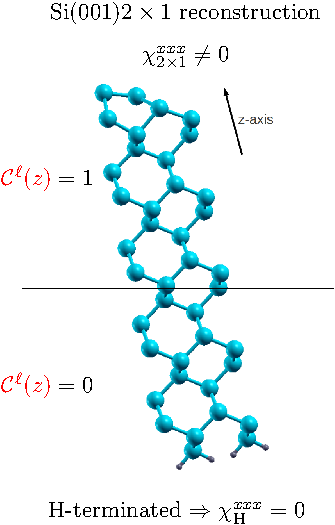
\includegraphics[scale=.8]{images/si2x1-crop}
\caption{(color on line) The slab shows a 
    clean Si(001)$2\times 1$ front surface 
    with an ideal terminated Si bulk back surface. The
    dangling bonds are H (small balls) saturated. 
    This image depicts 12 Si atomic layers
    with one H atomic layer. 
\label{si2x1}} 
\end{figure} 
The idea behind this slab configuration is that the 
cristalline symmetry of the H terminated surface imposes that 
$\chi_{\mathrm{H}}^{xxx}=0$.
 The $2\times 1$ surface has no 
such restrictions, so $\chi_{2\times 1}^{xxx}\ne 0$.
This is due to the fact that along the $y$ direction there is a mirror plane for the
H-saturated surface, whereas 
for the $2\times 1$ surface this mirror is lost as the dimers are
asymmetric along $x$. 
Thus, calculating $\chi^{xxx}$ for the full-slab, or the 
half-slab containing the $2\times 1$ surface\cite{nota1}
should yield the same result since the contribution from the H
saturated surface is zero regardless. 
We must check that the following 
relationship is satisfied for this particular slab
\begin{align}\label{hs}
\chi_{\mathrm{half-slab}}^{xxx}(-2\go;\go,\go) 
=
\chi_{\mathrm{full-slab}}^{xxx}(-2\go;\go,\go) 
,
\end{align}
where
$\chi_{\mathrm{half-slab}}^{xxx}(-2\go;\go,\go)$ is calculated using
$C(z)=1$ from the upper half containing the $2\times 1$ 
surface reconstruction, as seen in Fig.~\ref{si2x1},
and $\chi_{\mathrm{full-slab}}^{xxx}(-2\go;\go,\go)$ is calculated using
$C(z)=1$ through the full slab.
We show the results for this comparison in the remainder 
of this section


The self-consistent ground state and their Kohn-Sham states were
calculated in the DFT-LDA framework using the plane-wave 
ABINIT code.\cite{abinit}
We used Troullier-Martins pseudopotentials\cite{troullierPRB91} that are 
fully separable nonlocal pseudopotentials in the Kleinman-Bylander 
form.\cite{kleinmanPRL82}
The contribution of $\bfv^\nl$ to Eq.~\eqref{chis} can be carried out 
as detailed in Appendix \ref{vesnl} using the DP code for 
the actual calculation.\cite{francesco}
%
The surfaces have been studied with a lattice constant of 5.43 \AA. 
Structural optimizations were performed using DFT-LDA
with the ABINIT code.\cite{abinit}  
The geometry optimization as been carried out in slabs of 12
atomic layers where the central four layers where fixed at the bulk
positions.  
The structures were relaxed until the Cartesian force components were less and 5 meV/\AA. 
The geometry optimization for the clean surface gives
a dimer buckling of 0.721 \AA, and a dimer length of 2.301 \AA.  
For the  Si(001)$1\times 1$:2H dihydride surface, we have obtained a Si-H bond distance of 1.48 \AA. 
This results are in good agreement with previous 
theoretical studies.\cite{caramellaPRB09,mendozaPRB06}
%
The unit cell has two atoms making for a computationally
expensive calculation.
The vacuum size is equivalent to one quarter the
size of the slab, avoiding the effects produced by possible 
wave-function tunneling from the contiguous surfaces of the full
crystal formed by the repeated super cell scheme.\cite{mendozaPRB06}    

Spin-orbit, local field, and electron-hole 
attraction\cite{leitsmannPRB05,trollePRB14} 
effects on the SHG process are all neglected.
Although these are important factors in the optical response of a semiconductor,
their efficient calculation is still theoretically and  
numerically challenging and  
under debate. This merits further study but is beyond the scope of this paper.
For a given slab size, we find the converged spectra 
to obtain the relevant parameters. The most important of 
these are: an energy cut-off of 10 Ha, an equal number of conduction and 
valence bands, and a set of 244 $\bfk$-points.
The $\bfk$-points are used for the linear analytic 
tetrahedron method for evaluating the
Brillouin zone integrals in Eq.~\eqref{chis}, 
where special care was taken to examine the double resonances.\cite{nastosPRB05}
Double resonances occur at a given frequency $\omega$ if there can be 
resonant transitions at both $\omega$ and 2$\omega$ frequencies. This 
implies that there is a region in the Brillouin zone where 
$\omega_{cv}(\bfk)=2 \omega_{c'v}(\bfk)$. Since there is a real population 
excitation, the perturbation theory used to calculate the spectrum breaks 
down at these $\bfk$-points. This must be taken into account in a more 
complete calculation. These points introduce sharp spikes in the spectrum. 
In principle, these can affect the low frequency results since the response 
is computed from the Kramers-Kronig relation for frequencies below the band 
gap. However, in agreement with Ref.~\onlinecite{nastosPRB05} we find that 
the double resonances affect the low frequency results by less than 2\%. 
All spectra were calculated with a Gaussian smearing of 0.15 eV.
\begin{figure}
\centering 
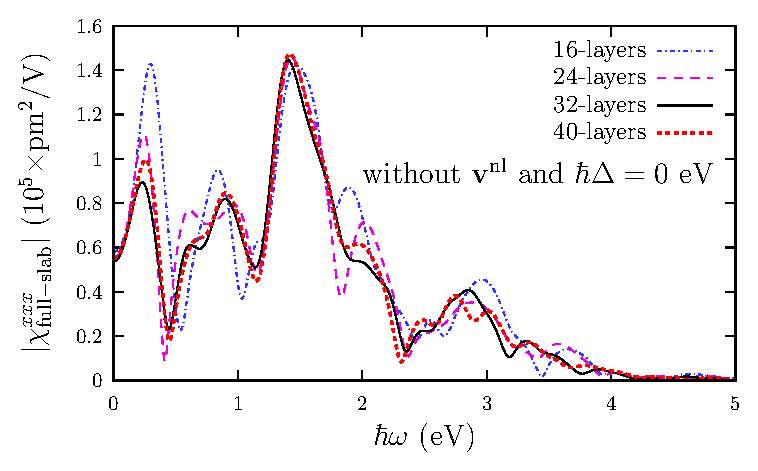
\includegraphics[scale=.8]{plots/fig1}
\caption{(color on line) 
$|\chi_{\mathrm{half-slab}}^{xxx}|$ vs $\hbar\omega$ 
for the slab
with 16, 24, 32, and 40 atomic Si layers. The front surface 
is in a clean $2\times 1$ reconstruction and the back 
surface is an ideal terminated bulk H-saturated dangling bonds.
\label{fig1}} 
\end{figure}
\begin{figure}
\centering 
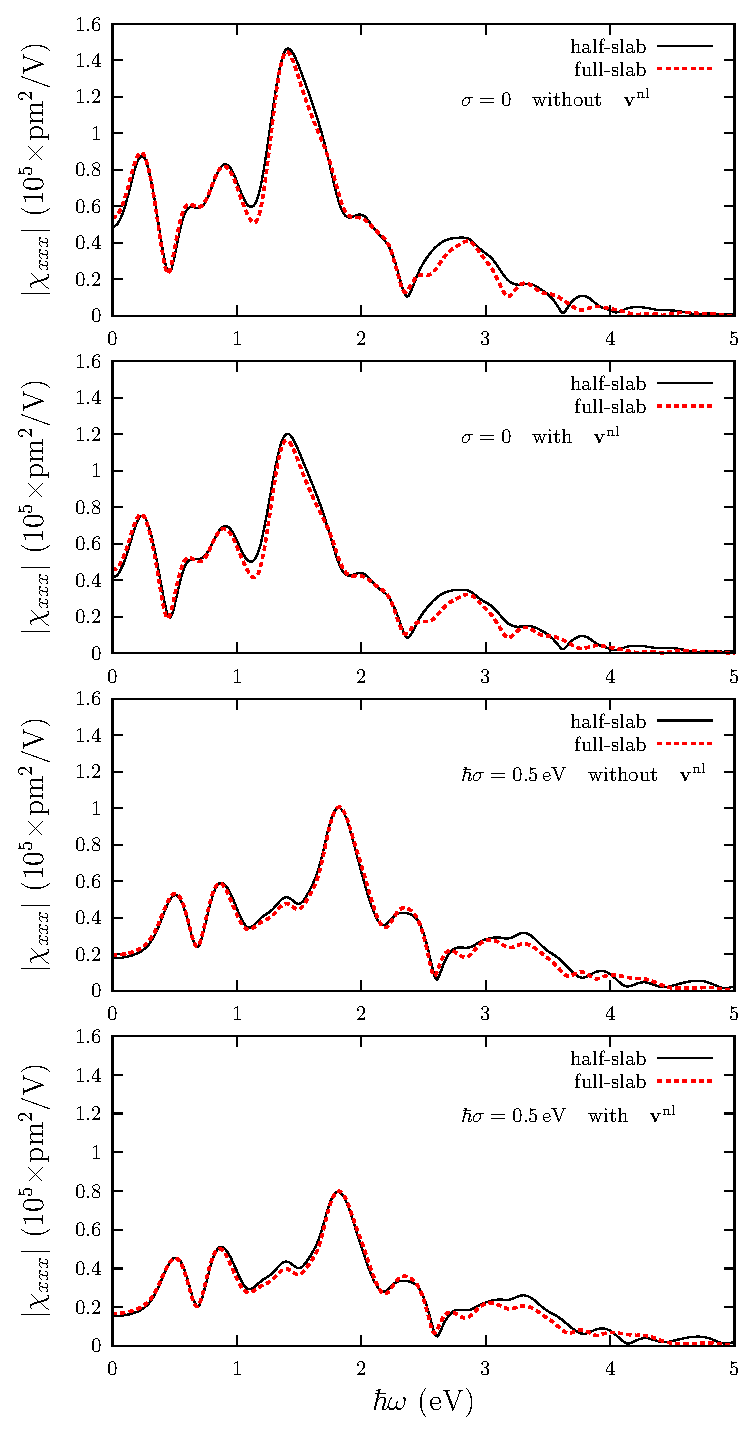
\includegraphics[scale=.8]{plots/fig2}
\caption{(color on line) 
$\chi^{xxx}_{\mathrm{half-slab}}$
and 
$\chi^{xxx}_{\mathrm{full-slab}}$
vs $\hbar\omega$ for a slab with 32 
atomic Si layers plus one H layer. 
\label{fig2}} 
\end{figure}

We must evaluate 
$T^{\rma\rmb}_{nm}=(i/\hbar)[r^\rmb,v^{\nl,\rma}]_{nm}$,
as outlined in Appendix \ref{vesnl},
in order to obtain 
Eqs.~\eqref{tau.1} and \eqref{tau.1n} that are required for 
Eq.~\eqref{chis}.
Computing second 
order derivatives is required thus making the numerical procedure very 
time consuming. This adds significantly to the already lengthy time needed 
for the calculation of the $\bfv^\nl$ contribution that is
proportional only to 
the first order derivatives. 
Memory requirements are also increased for both $\bfv^\nl$ and 
$[\bfr,\bfv^\nl]$. However, the contribution from $[\bfr,\bfv^\nl]$ 
is very small\cite{valerie} and therefore we neglect it in this work.

\subsection{Full-slab results}\label{fsresults}

In Fig.~\ref{fig1} we show $|\chi_{\mathrm{full-slab}}^{xxx}|$
for the slab with
16, 24, 32, and 40 Si atomic layers. 
We note that the response differs substantially 
for 16 and 24 layers but is quite similar for 32 and 40 layers.
As explained above,
the calculation of the $\bfv^\nl$ contribution is 
computationally expensive.
A good compromise between the accuracy in the convergence of
$\chi^{xxx}_{\mathrm{full-slab}}$ as a function of the number
of layers in the slab, and the computational 
expense is to consider
the slab with 32 Si atomic layers as 
an accurate representation of our 
system.

\subsection{Half-slab vs. full-slab}

In Fig.~\ref{fig2}
we compare 
$\chi^{xxx}_{\mathrm{half-slab}}$  
vs. 
$\chi^{xxx}_{\mathrm{full-slab}}$ 
for the four different possibilities 
between including or not including the
effects of $\bfv^\nl$ or the scissors correction
$\hbar\sigma$.   
For these results we chose
$\hbar\sigma=0.5$ eV, that is the GW gap reported in
Ref.~\onlinecite{rholfingPRB95,garciaCPC01}. 
We see that for all four instances the 
difference between responses is quite small.
Indeed, when the value $|\chi^{xxx}|$ 
is large the difference between the two is very small; 
when the value is small the difference increases only slightly, 
but the spectra is so close to zero that these it is negligible. 
These differences would decrease as the number of atomic layers 
increases. We remark that 32 layers in the slab is more than enough 
to confirm that the extraction of the surface second harmonic 
susceptibility from the $2\times 1$ surface is readily possible 
using the formalism contained in Eq.~\eqref{chis}.
This confirms the validity of our theory and is the main result of
this article; through the proposed layer formalism we can calculate the surface SH
susceptibility including the effect of the non-local part of the
pseudopotentials
and the many-body effects through the scissors correction.
Our scheme ought to work for any slab.  

\subsection{\texorpdfstring{Results for $\chi^{xxx}_{2\times 1}(-2\go;\go,\go)$}{Results for Xxxx(2x1)(-2w;w,w)}}

We proceed to explain 
some of the features seen in $|\chi^{xxx}_{2\times 1}|$ that, as
explained above, are obtained 
by calculating $|\chi^{xxx}_{\mathrm{half-slab}}|$.
First, from Fig.~\ref{fig2} we note a series of resonances 
that derive from 1$\omega$ and 2$\omega$ terms in
Eq.~\eqref{chis}. 
Notice that the 
2$\omega$ resonances start below $E_g/2$ where $E_g=??$ eV is the LDA
band gap of this surface, and $E_g=??$ eV is the scissor shifted gap for
$\hbar\sigma=0.5$ eV.
These resonances
come from the electronic states of the 
$2\times 1$ surface, that lie inside the bulk band gap of Si and are the 
well known electronic surface states.
In Fig.~\ref{fig3}
We see that the effect of $\bfv^\nl$ reduces the value of   
$|\chi^{xxx}_{2\times 1}|$,
without changing the 
spectral shape; this also can be confirmed from
the cases of zero scissors correction from Fig.~\ref{fig2}.
%
From Fig.~\ref{fig4}
we note that the scissors correction 
shifts the spectra to higher energies as expected. However, contrary 
to the case of linear optics\cite{cabellosPRB09} the shift introduced
by the scissors correction is not 
rigid, as pointed out in Ref.~\onlinecite{nastosPRB05}.
 This is because the second harmonic optical response mixes 
$1\omega$ and $2\omega$ transitions (see Eq.~\eqref{chis}), and accounts 
for the non-rigid shift.
\begin{figure}
\centering 
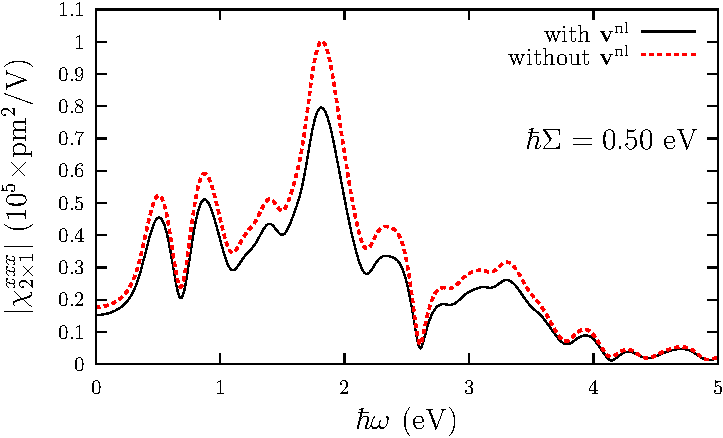
\includegraphics[scale=.8]{plots/fig3}
\caption{(color on line) 
$\chi^{xxx}_{2\times 1}$
vs $\hbar\omega$ for a slab with 32 
atomic Si layers plus one H layer, 
with and without the contribution from $\bfv^\nl$.
\label{fig3}} 
\end{figure}
\begin{figure}
\centering 
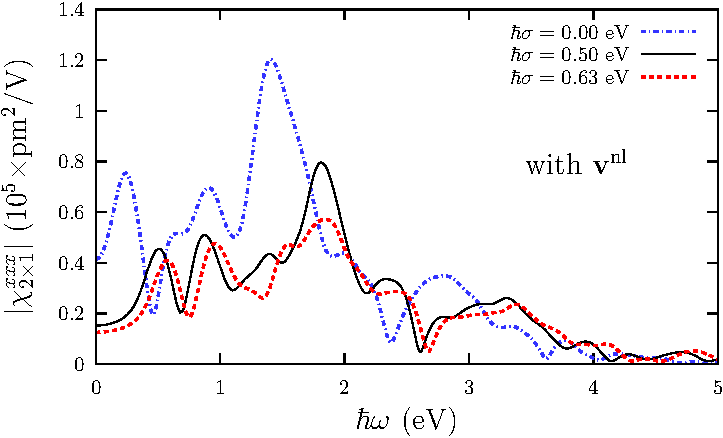
\includegraphics[scale=.8]{plots/fig4}
\caption{(color on line) 
$\chi^{xxx}_{2\times 1}$
vs $\hbar\omega$ for a slab with 32 
atomic Si layers plus one H layer, 
for two different values of 
the scissors correction $\hbar\sigma$. 
\label{fig4}} 
\end{figure}
Also, when we compare 
$|\chi^{xxx}_{2\times 1}|$ for two values of $\hbar\sigma$,
we see that the first two peaks are almost rigidly 
shifted with a small difference in height while
the rest of the peaks are modified substantially. 
This behavior comes from the fact that the first two
peaks are almost exclusively related to the 
2$\omega$ resonances of
Eq.~\eqref{chis}. The other peaks are a combination 
of 1$\omega$ and 2$\omega$ resonances 
and yield a more varied spectrum. 
This way we see that small changes in the value of the 
scissors shift can in general affect the SSH susceptibility 
spectrum quite dramatically.
We mention that
the value of $\hbar\sigma=0.5$ eV, used above, 
is the ``average'' GW gap taken from 
Ref.~\onlinecite{rholfingPRB95} 
that is in agreement with Ref.~\onlinecite{garciaCPC01}. 
The value of $\hbar\sigma=0.63$ eV is the ``average'' 
gap taken from Refs.~\onlinecite{asahiPRB00}, 
where more $\bfk$-points in the Brillouin zone were
used to calculate its GW value.

Although, local fields are neglected, we expect that parallel to an
interface they should be in principle 
small, as the electric field is continuous. So, we would expect that the $xxx$ component 
of 
$\bfgchi(-2\go;\go,\go)$, would have an small influence from the local fields.
Unfortunately the experimental measurement of the $xxx$
component of $\bfgchi(-2\go;\go,\go)$ is not possible, as the SH 
radiated intensity would be proportional not only to this component 
but also to other components of $\bfgchi(-2\go;\go,\go)$,  
however,
in a forthcoming publication 
we will present a study of SSHG from several 
Si surfaces 
with comparison to experimental 
results. 

\section{Conclusions}\label{conc}

We have presented a formulation to calculate surface second harmonic
(SSH) susceptibility tensor $\bfgchi(-2\go;\go,\go)$,  using a length gauge
formalism and within the independent particle approximation (IPA).
It includes on the same footing and for the first time in the literature 
i) the scissors correction, ii) the cut function, and iii) the 
contribution of the non-local part of the pseudopotentials. 
We have used a Si(001)$2\times 1$ surface to confirm that our scheme
correctly obtains the surface response as we confirm
that 
$\chi_{\mathrm{half-slab}}^{xxx}(-2\go;\go,\go) 
\approx
\chi_{\mathrm{full-slab}}^{xxx}(-2\go;\go,\go) 
. 
$
Although, one can in principle increase the number of atomic layers,
$\bfk$-points, etc.  to
improve even further on the similarity of the half-slab and full-slab results, we
hava chosen a good compromise between accuracy and the burden and time
of the computational scheme. 
We describe the effect of the independent inclusion of the three
effects mentioned above in the calculation of  
$\bfgchi(-2\go;\go,\go)$. To wit,
the scissors correction shifts the spectrum to higher energies, though
the shifting is not rigid and mixes the 1$\omega$ and 2$\omega$
resonances, the cut functions
allow us
to extract unequivocally   
$\chi^{xxx}_{2\times 1}(-2\go;\go,\go)$, 
and the effects of the nonlocal part of the pseudopotentials,
reduces the value of   
$|\chi^{xxx}_{2\times 1}(-2\go;\go,\go)|$, keeping the same lineshape. 
The $xxx$ component of  
$\bfgchi_{2\times 1}(-2\go;\go,\go)$, 
could not be
experimentally  isolated,
however in a forthcoming publication 
we will compare our formulation 
against
experimental 
results. 
We have neglected
local field 
and excitonic effects.
Although these are important factors in the optical response of a semiconductor,
their efficient calculation is theoretically and 
numerically challenging and still 
under debate.\cite{beyond}  
This merits further study but is beyond the scope of this paper. 
Nevertheless, the inclusion of aforementioned contributions 
in
our scheme opens the unprecedented possibility to study 
surface SHG with more versatility and providing 
more accurate results than previous approaches. 





%%%%%%%%%%%%%
\appendix 
\section{}\label{appe}
We give explicit expressions for the quantities used in the evaluation 
of Eq.~\eqref{chis}; when appropriate, some 
intermediate steps are given for their derivation. 
%%%%
\subsection{ Expressions for 
\texorpdfstring{${\calbv}_{nm}(\bfk)$}{que} 
and 
\texorpdfstring{${\cal C}_{nm}(\bfk)$}{que}
}\label{calpcalc}

Expanding the wave function in plane waves we obtain
\begin{align}\label{eni.1}
\psi_{n\bfk}(\bfr)=\sum_\bfG A_{n\bfk}(\bfG)e^{i(\bfk+\bfG)\cdot\bfr}
,
\end{align}
where $\{\bfG\}$ are the reciprocal basis vectors satisfying
$e^{\bfR\cdot\bfG}=1$, with $\{\bfR\}$ the translation vectors in real
space, and $A_{n\bfk}(\bfG)$ the expansion coefficients. Using
$m_e\bfv=\bfp=-i\hbar\bfgnabla$ into 
Eq.~\eqref{vcali}
we obtain,\cite{mendozaPRB06}
\begin{align}\label{eni.2}
\calbv_{nm}(\bfk)=
\frac{\hbar}{2m_e}
\sum_{\bfG,\bfG'} A^*_{n\bfk}(\bfG')  A_{m\bfk}(\bfG)
(2\bfk+\bfG+\bfG')
\gd_{\bfG_\parallel \bfG'_\parallel}  
f(G_\perp-G'_\perp)
,
\end{align}   
where
\begin{align}\label{vnl.9}
f(G_\perp)=\frac{1}{L}\int\calc(z) e^{iG_\perp z}dz  
 ,
\end{align}
with $f^*(G_\perp)=f(-G_\perp)$,
and $L$
is the length of the super cell. 
The reciprocal lattice vectors $\bfG$ are 
decomposed into components
parallel ($\bfG_\parallel$), and perpendicular ($G_\perp \hat z$)
to the surface, so
that $\bfG = \bfG_\parallel + G_\perp\hat z$.
The double summation over the $\bfG$ vectors can be 
calculated efficiently by  
creating a pointer array to identify all the plane-wave coefficients  
associated with the same $G_\parallel$.  

Likewise we obtain that
\begin{align}\label{eni.4}
\calc_{nm}(\bfk)=
\sum_{\bfG,\bfG'} A^*_{n\bfk}(\bfG')  A_{m\bfk}(\bfG)
\gd_{\bfG_\parallel \bfG'_\parallel} 
f(G_\perp-G'_\perp)
.
\end{align}  
If $\calc(z)=1$, then $f(G_\perp)=\gd_{G_\perp 0}$ and we 
obtain the full-slab/bulk values, 
$\bfv_{nm}(\bfk)$ and $\calc_{nm}(\bfk)=\gd_{nm}$,
from Eqs.~\eqref{eni.2} and \eqref{eni.4}.

%%%%
\subsection{Expressions for 
\texorpdfstring{$(\calv^{\lda,a}_{nm})_{;k^b}$}{Vnonlocal},
\texorpdfstring{$(r^a_{nm})_{;k^b}$}{Vnonlocal}
and \texorpdfstring{$(\calc_{nm})_{;\bfk}$}{Vnonlocal}
}\label{appvnl}

Using Eqs.~\eqref{rnminn}, \eqref{conmri3n}, \eqref{gendevnn}, and
defining 
$
\calt^{\rma\rmb}\equiv[r^{\rmb},\calv^{\lda,\rma}]
\equiv
[r^{\rmb},\calv^\rma]
$
one can show that
\begin{align}\label{nmesn}
(\calv^{\lda,\rma}_{nm})_{;k^{\rmb}}&=
\calt_{nm}^{\rma\rmb}
+i
\sum_{q}
\bigg(
r^{\rmb}_{nq}  
\calv^{\lda,\rma}_{q m}
-
\calv^{\lda,\rma}_{nq}   
r^{\rmb}_{q m}
\bigg)  
+i  
r^{\rmb}_{nm}
\Delta^{\rma}_{mn}
,
\end{align}
where
\begin{eqnarray}\label{tdel}
\Delta^{\rma}_{mn}
=
\calv^{\lda,\rma}_{nn}  
-
\calv^{\lda,\rma}_{mm}  
,
\end{eqnarray} 
\begin{align}\label{tau.1}
\calt_{nm}^{\rma\rmb}
=
\frac{\hbar}{m_e}\gd_{\rma\rmb} 
C_{nm} 
-\hbar 
\sum_q  
L^{\rma\rmb}_{nq} 
C_{qm} 
,
\end{align}   
and
\begin{align}\label{lab}
L_{nm}^{\rma\rmb}
=\frac{i}{\hbar}[r^{\rmb},v^{\nl,\rma}]_{nm}
.
\end{align}  
The matrix elements $L^{\rma\rmb}_{nm}$
are calculated in Appendix \ref{vesnl}.
% is small
%compared to the other terms, thus we neglect it throwout this work.\cite{valerie} 
Notice that
$(v^{\lda,\rma}_{nm})_{;k^{\rmb}}$ is obtained 
from Eq.~\eqref{nmesn} by 
taking 
$C(z)=1$ or $C_{nm}=\gd_{nm}$.

To obtain $(r^{\rma}_{nm})_{;k^{\rmb}}$ we use Eq.~\eqref{chon.10} to
write
$(r^{\rma}_{nm})_{;k^{\rmb}}
=(v^{\lda,\rma}_{nm}/i\go^\lda_{nm})_{;k^{\rmb}}
$ and simply apply the chain rule,
\begin{align}\label{rka}
(r^{\rma}_{nm})_{;k^{\rmb}}
&=
T^{\rma\rmb}_{nm}
+
\frac{ 
r^{\rmb}_{nm}
\Delta^{\rma}_{mn}
+r^{\rma}_{nm}
\Delta^{\rmb}_{mn}
}
{\go^\lda_{nm}}
+
\frac{i}{\go^\lda_{nm}}
\sum_{q}
\bigg(
\go^\lda_{q m} 
r^{\rmb}_{nq} 
r^{\rma}_{q m}
-
\go^\lda_{nq} 
r^{\rma}_{nq} 
r^{\rmb}_{q m}
\bigg)
,
\end{align} 
where 
\begin{eqnarray}\label{del}
\Delta^{\rma}_{mn}
=
v^{\lda,\rma}_{nn}  
-
v^{\lda,\rma}_{mm}  
,
\end{eqnarray}
and
\begin{align}\label{tau.1n} 
T_{nm}^{\rma\rmb}
=\frac{\hbar}{m_e}\gd_{ab}\gd_{nm} 
-\hbar L^{\rma\rmb}_{nm} 
.
\end{align}
Eq.~\eqref{rka} generalizes the usual expresion of
$(r^a_{nm})_{;k^b}$ for a local 
Hamiltonian
\cite{aversaPRB95,nastosPRB05,cabellosPRB09,rashkeevPRB98}
to
the case of a
nonlocal Hamiltonian.
Note that the layered term
$\calt^{\rma\rmb}_{nm}$ reduces to $T^{\rma\rmb}_{nm}$
for the full-slab/bulk case.

Again, we use Eqs.~\eqref{rnminn}, \eqref{conmri3n}, and \eqref{gendevnn},
along with $[\bfr,F(\bfr)]=0$, valid for 
and any function $F(\bfr)$, 
to obtain 
\begin{align} 
(\calc_{nm})_{;\bfk}
&=
i 
\sum_{q} 
 \left(\bfr_{nq}
\calc_{qm}
-
\calc_{nq}
\bfr_{qm}
\right) 
+i\bfr_{nm}(\calc_{mm}-\calc_{nn}) 
,
\end{align} 
where we remind the reader that $\bfr_{nm}$ 
is calculated through 
Eq.~\eqref{chon.10} for LDA. 


%%%%
\subsection{
\texorpdfstring{$\calbv^{\nl}_{nm}$}{Vnonlocal},
\texorpdfstring{$\bfv^\nl_{nm}$}{Vnonlocal}, and 
\texorpdfstring{$T^{\rma\rmb}_{nm}$}{[r,vnl]}}
\label{vesnl}

We take Eq.~\eqref{vnl} into Eq.~\eqref{vcali}
and use
$\sum_{\bfG}\ket{\bfk+\bfG}\bra{\bfk+\bfG}=1$, 
with
$\braket{\bfr}{\bfk+\bfG}=(1/\sqrt{\gO})
\mathrm{exp}(i(\bfk+\bfG)\cdot\bfr)$
to obtain,
\begin{align}\label{vnl.5}
\calbv^{\nl}_{nm}(\bfk)&=\frac{1}{2}
\sum_{\bfG}
\Big(
\bra{n\bfk} C(z) 
\ket{\bfk+\bfG}\bra{\bfk+\bfG}
\bfv^\nl \ket{m\bfk}
+
\bra{n\bfk}
\bfv^\nl  
\ket{\bfk+\bfG}\bra{\bfk+\bfG}
C(z) \ket{m\bfk}
\Big)
\nonumber\\
&=\frac{1}{2 \hbar}
\sum_{\bfG}
\left(
\calf^{\ell*}_{n\bfk}(\bfG) 
H_{m\bfk}(\bfG) 
+
H^*_{n\bfk}(\bfG) 
\calf_{m\bfk}(\bfG) 
\right) 
,
\end{align}  
where 
we have defined  
\begin{align}\label{vnl.10}
\calf_{n\bfk}(\bfG) 
=
\sum_{\bfG'} 
A_{n\bfk}(\bfG') 
\gd_{\bfG_\parallel \bfG'_\parallel}f(G'_\perp-G_\perp) 
,
\end{align} 
\begin{align}\label{vnl.11}
H_{n\bfk}(\bfG)&=
\sum_{\bfG'} 
A_{n\bfk}(\bfG') 
(\nabla_{\bfK}+\nabla_{\bfK'})  
V^\nl(\bfK,\bfK')
,
\end{align}
and $\bfK=\bfk+\bfG$, $\bfK'=\bfk+\bfG'$.
For fully  separable pseudopotentials in the   
Kleinman-Bylander (KB) form,\cite{mottaCMS10,kleinmanPRL82,adolphPRB96}  
the  
matrix elements 
 $\bra{\bfK}  
V^\nl  
\ket{\bfK'}
=V^\nl(\bfK,\bfK')  
$ 
and their $\bfK$ and $\bfK'$ gradient 
can be readily calculated.\cite{mottaCMS10,adolphPRB96,gordienkoRPJ04,fuchsCPC99} 
We have 
implemented 
the calculation of $\calbv^{\nl}_{nm}(\bfk)$ with the help of 
the \depe~code.\cite{francesco}
We obtain $\bfv^{\nl}_{nm}(\bfk)$ from the previous three 
expressions by taking $C(z)=1$, which implies 
that $f(G_\perp)=\gd_{G_\perp 0}$, 
and 
$\calf_{n\bfk}(\bfG) \to F_{n\bfk}(\bfG)=A_{n\bfk}(\bfG)$.

From Eqs.~\eqref{lab} and \eqref{vnl} 
\begin{align}\label{3.1}
L^{\rma\rmb}_{nm}(\bfk) 
=
\frac{1}{\hbar^2}
\bra{n\bfk}
\big[ r^{\rma},[ V^\nl, r^\rmb]\big]
\ket{m\bfk}
,
\end{align} 
and we expand the triple commutator to obtain,
\begin{align}\label{3.5}
L^{\rma\rmb}_{nm}(\bfk) 
&=
\frac{1}{\hbar^2\gO}
\sum_{\bfG,\bfG'} 
A^*_{n\bfk}(\bfK) 
A_{m\bfk}(\bfK')
\int
d\bfr d\bfr'
 e^{-i\bfK\cdot\bfr}
\Big(
r^{\rma}
V^\nl(\bfr,\bfr')
r'^\rmb
-
V^\nl(\bfr,\bfr')
r'^\rma
r'^{\rmb}
\nonumber\\
&-
r^\rmb
r^{\rma}
V^\nl(\bfr,\bfr')
+
 r^\rmb
V^\nl(\bfr,\bfr')
r'^{\rma}
\Big) 
 e^{i\bfK'\cdot\bfr'}
,
\end{align} 
where 
$V^\nl(\bfr,\bfr') = \bra{\bfr} V^\nl\ket{\bfr'}$.
We use the following identity
\begin{align}\label{3.4}
&
\Big(
\frac{\partial^2}{\partial K^\rma\partial K'^\rmb}
+
\frac{\partial^2}{\partial K'^\rma\partial K'^\rmb}
+
\frac{\partial^2}{\partial K^\rma\partial K^\rmb}
+
\frac{\partial^2}{\partial K^\rmb\partial K'^\rma}
\Big)
\int 
d\bfr d\bfr' 
 e^{-i\bfK\cdot\bfr}
V^\nl(\bfr,\bfr') 
e^{i\bfK'\cdot\bfr'}
\nonumber\\
&=
\int d\bfr d\bfr'
 e^{-i\bfK\cdot\bfr}
\Big( 
r^{\rma} 
V^\nl(\bfr,\bfr') 
r'^\rmb
- 
V^\nl(\bfr,\bfr') 
r'^\rma 
r'^{\rmb}
- 
r^\rmb 
r^{\rma} 
V^\nl(\bfr,\bfr')
+
 r^\rmb 
V^\nl(\bfr,\bfr') 
r'^{\rma}
\Big)  
e^{i\bfK'\cdot\bfr'}
,
\end{align}
to write
\begin{align}\label{3.7}
L^{\rma\rmb}_{nm}(\bfk)
&=
\frac{1}{\hbar^2}
\sum_{\bfG,\bfG'} 
A^*_{n\bfk}(\bfK) 
A_{m\bfk}(\bfK')
\Big(
\frac{\partial^2}{\partial K^\rma\partial K'^\rmb}
+
\frac{\partial^2}{\partial K'^\rma\partial K'^\rmb}
+
\frac{\partial^2}{\partial K^\rma\partial K^\rmb}
+
\frac{\partial^2}{\partial K^\rmb\partial K'^\rma}
\Big)
\bra{\bfK} 
V^\nl 
\ket{\bfK'}, 
\nonumber\\
\end{align} 
where
\begin{align}\label{vkk}
\bra{\bfK} 
V^\nl 
\ket{\bfK'} 
=
\frac{1}{\gO}
\int 
d\bfr d\bfr' 
 e^{-i\bfK\cdot\bfr}
V^\nl(\bfr,\bfr') 
e^{i\bfK'\cdot\bfr'}
,
\end{align}
The double derivatives with respect to $\bfK$ and $\bfK'$ 
can be worked out explicitly and 
$L^{\rma\rmb}_{nm}(\bfk)$
can be finally calculated.\cite{valerie}

%%%%
\subsection{Expressions for  \texorpdfstring{$\calbv^{S}_{nm}$}{Vnm}
and
\texorpdfstring{$\Big({\calbv}^{S}_{nm}\Big)_{;\bfk}$}{(Vnm);kb}
}\label{calvs} 

From Eq.~\eqref{vcali}
\begin{align}\label{a.3b}
\calbv^{S}_{nm}
&=
\frac{1}{2}\sum_q\left(   
\bfv^S_{nq}\calc_{qm}+\calc_{nq}\bfv^S_{qm}
\right)  
,
\end{align}    
where $\sum_q\ket{q\bfk}\bra{q\bfk}=1$ was used
and $\bfv^S_{nm}$ is given in Eq.~\eqref{chon.2}.
Taking the generalized derivative of Eq.~\eqref{a.3b}
and applying
the chain rule, we obtain
\begin{align}\label{a.3bn}
\left(\calbv^{S}_{nm}\right)_{;\bfk}
&=
\frac{1}{2}\sum_q\left(
(\bfv^S_{nq})_{;\bfk}\calc_{qm}
+    
\bfv^S_{nq}(\calc_{qm})_{;\bfk}
+
(\calc_{nq})_{;\bfk} \bfv^S_{qm}
+
\calc_{nq} (\bfv^S_{qm})_{;\bfk}
\right)  
.
\end{align}    
Again, from
Eq.~\eqref{chon.2}, 
\begin{align}\label{choni.1}
(\bfv^S_{nm})_{;\bfk}=i\gs f_{mn}
(\bfr_{nm})_{;\bfk}
,
\end{align}
a result that is in agreement with Eq. A(6) of Ref.~\onlinecite{cabellosPRB09}.

%%%%%%%%%%%%%%
\newpage
\bibliography{ref}% 
\end{document}  %
%%%%%%%%%%%%%%


\section{Introduction}\label{intro}

The first attempt to go beyond the independent particle approximation 
could be found in 
Leitsmann \textit{et al}.\cite{leitsmannPRB05} 
that included excitonic and local field interactions. 
More recently, Luppi \textit{et al.}\cite{luppiPRB10,luppiJCP10} and 
H\"ubner \textit{at al.}\cite{hubenerPRB11}, studied 
the influence of crystal local fields and excitonic effects on 
the spectrum of the second harmonic generation of several bulk 
systems 
by using time-dependent density-functional theory 
including many-body effects, namely, quasiparticle corrections through 
the scissors operator, crystal local field effects, and excitonic 
interaction.  
Also,
Trolle \textit{et al}.\cite{trollePRB14} 
elaborate on a theoretical model for SHG of 
mono-layer MoS$_{2}$. Their approach is based on the tight-binding model 
fitted to GW results and include excitonic effects from the 
Bethe-Salpeter exciton picture. However, neither of these models 
has a consideration for surfaces. 
